\chapter{Results}

This chapter presents the experimental results obtained from the proposed EEG-based
system. The work has two parts and the results follow the same split. The first part deals
with motor imagery, where the aim is to find out whether EEG recorded from a four-channel
dry headset carries enough information to tell a left-hand imagination apart from a
right-hand one. The second part deals with cognitive assessment, where the aim is to
compute attention, cognitive load, relaxation, stress and fatigue from the frequency bands
of the same signal. Results are reported in the order the work was carried out, starting
with the reproduction of the stroke dataset analysis, then the same analysis and a set of
classifiers on the BCI Competition IV 2b dataset of healthy subjects, then the analysis of
the data recorded in this project and its classifier, and finally the cognitive scoring
system.

\section{Evaluation Aspects}

For the motor imagery part, the EEG signals recorded during imagined left-hand and
right-hand grasps are compared in the time domain, through event-related desynchronisation
and synchronisation (ERD/ERS), and through power spectral density (PSD). These analyses
check whether the two classes show any consistent difference that a classifier can use. For
the cognitive part, the relative power in each frequency band is tracked over a session and
converted into scores, and the stability of the recording itself is checked through the
electrode impedance.

\subsection{Cases of Comparison}

The following comparison cases were studied during the experimental analysis:

\begin{enumerate}
    \item ERD/ERS of the stroke reference dataset, reproduced to validate the analysis method
    \item ERD/ERS, PSD, C3/C4 power ratio and SVM accuracy on the BCI Competition IV 2b
          dataset of healthy subjects
    \item ERD/ERS of the data recorded in this project, compared against the reference
    \item PSD of C3 and C4 for imagined left versus imagined right
    \item Classification accuracy of different SVM feature sets and kernels
    \item Band power and cognitive scores recorded over a complete session
\end{enumerate}

\subsection{Parameters Under Study}

The main parameters considered in this analysis are:

\begin{enumerate}
    \item EEG channels: C3, C4, A1 and A2, with C3 and C4 as the motor cortex pair
    \item Motor imagery classes: imagined left-hand grasp and imagined right-hand grasp
    \item Frequency range: 8--30 Hz for motor imagery, 1--30 Hz for cognitive scoring
    \item Features: band power, C3/C4 power ratio, mean, median, skewness and kurtosis
    \item Cognitive outputs: attention, cognitive load, relaxation, stress and fatigue
\end{enumerate}

\section{Experimental Setup}

The experiment was carried out using the GELO BCI headset with four EEG channels and one
reference electrode, sampling at 250 Hz. The acquisition was done through the Capsule GUI,
shown in Figure~\ref{fig:gui_acquisition}. Before every session the headset was paired over
Bluetooth, the electrode resistances were checked, and the two calibration steps described
in Chapter 5 were performed.

\begin{figure}[!htbp]
    \centering
    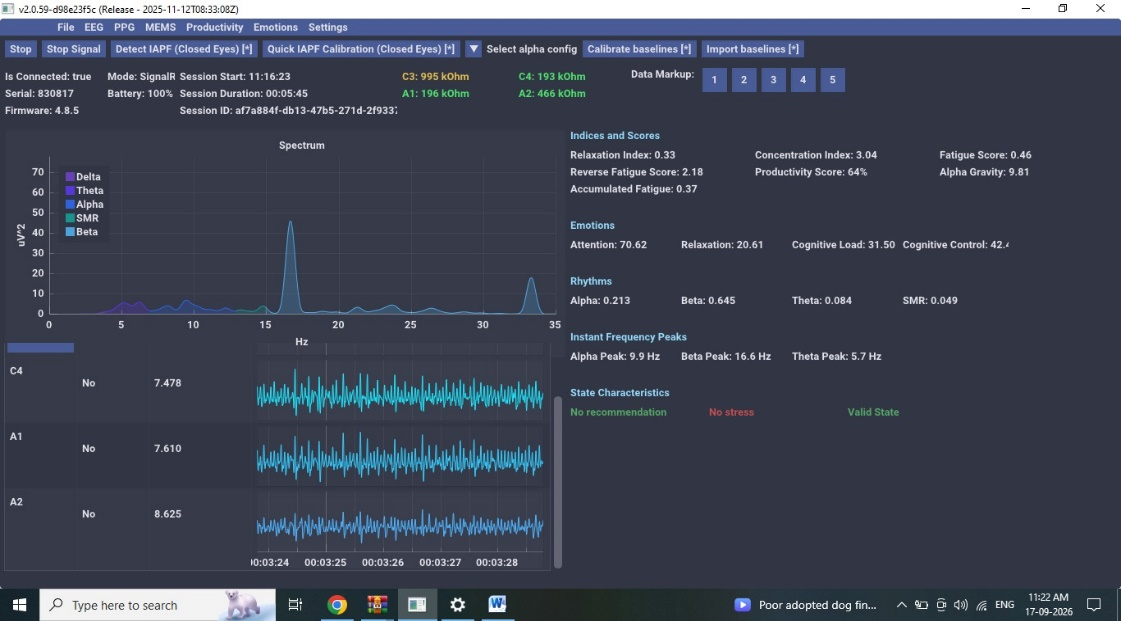
\includegraphics[width=0.85\linewidth]{gui_acquisition.jpg}
    \caption{EEG signal acquisition using the Capsule GUI}
    \label{fig:gui_acquisition}
\end{figure}

During each recording session the subject was seated comfortably and asked to imagine
gripping an object with the left hand or the right hand when prompted. The movement was
only imagined, so no actual movement was made. Each imagination was marked in real time
using a marker, which was recorded alongside the EEG so that the start and end of every
trial could be identified later. Each recorded file contains five marked repetitions of one
class. The session was saved in \texttt{.h5} format and converted to CSV for processing.

For post-recording analysis the CSV files were loaded and sorted by class based on their
filenames. The marker column was used to extract the active imagination windows as
individual trials. Since the shortest trial across the recordings was close to four
seconds, a fixed window of four seconds from the onset of each imagination was used so that
every trial contributes the same number of samples. The signal supplied by the device is
already filtered, so no further filtering was applied before the feature calculation except
the 8--30 Hz band limiting used for the ERD and PSD analysis. PSD was estimated using
Welch's method \cite{welch1967} with a window size of 256 samples at $F_s = 250$ Hz. Out of all the
recordings made, 50 right-hand trials and 22 left-hand trials were found usable, the rest
being discarded because of poor electrode contact or movement during the trial.

\FloatBarrier

\section{Reproduction of the Stroke Dataset Analysis}
\label{sec:stroke_repro}

Before working on the recorded data, the ERD/ERS analysis of the reference
dataset~\cite{liu2024mi} was reproduced. This was done to confirm that the analysis method
used in this project gives the same result as the published work before it is applied to
new data. Event-related desynchronisation refers to a drop in EEG power in a given
frequency band during a task, and event-related synchronisation refers to a rise
\cite{pfurtscheller1999erd}. For motor
imagery, power in the 8--30 Hz range is expected to fall over the hemisphere opposite to
the imagined hand.

The C3 and C4 signals were extracted, filtered between 8 and 30 Hz using a second-order
zero-phase Butterworth filter, squared to obtain power, averaged across trials, and
smoothed. The change was computed as

\begin{equation}
\mathrm{ERD/ERS}~(\%) = \frac{X - M}{M} \times 100
\end{equation}

where $X$ is the power at a given instant and $M$ is the average power during the one
second preparation period before the task. Figure~\ref{fig:erd_paper} shows the result
obtained for subject 8 of the dataset. During left-hand imagery the C4 trace separates
clearly from C3 and falls through the middle of the trial, which is the expected
contralateral response. During right-hand imagery the two traces stay much closer together.
This matches the behaviour reported in the dataset paper and confirms that the processing
chain is correct.

\begin{figure}[!htbp]
    \centering
    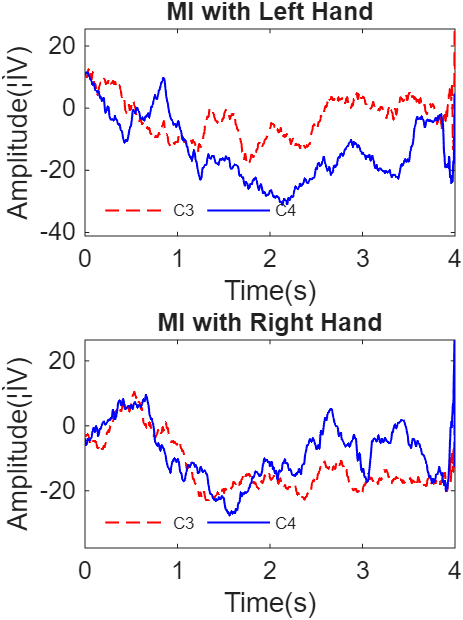
\includegraphics[width=0.45\linewidth]{erd_paper.png}
    \caption[ERD/ERS of C3 and C4 for subject 8 of the reference dataset]%
            {ERD/ERS of C3 and C4 for subject 8 of the reference dataset~\cite{liu2024mi},
             reproduced using the analysis method of this project}
    \label{fig:erd_paper}
\end{figure}

\FloatBarrier

\section{Results on the BCI Competition IV 2b Dataset}
\label{sec:bci2b}

The stroke dataset turned out to be a hard place to start. Even the published methods,
using all 30 channels, reach only 55 to 72 per cent on it~\cite{liu2024mi}, so a low score
there cannot tell us whether our own processing is right or wrong. A second reference was
needed, one that is closer to the GELO headset. The BCI Competition IV 2b dataset, called
the BCI 2008 dataset in this report and described in Section~\ref{sec:mi_datasets}, fits
this need well: the subjects are healthy, the sampling rate is 250 Hz, and the electrodes
sit at C3 and C4 just like on the headset. Every step in this section uses the same
method that was used for the stroke patients, so that the two can be compared directly.

\subsection{How the Dataset Was Used}

The dataset was downloaded as 18 MATLAB files, one training file and one evaluation file
for each of the nine subjects. The training file holds sessions 1 to 3 and the evaluation
file holds sessions 4 and 5. Each file contains the continuous EEG of the three channels
(C3, Cz and C4) and the three EOG channels, the sample number at which every trial starts,
the class of every trial (1 for left hand, 2 for right hand), and a flag that the dataset
authors set on trials they found to contain artefacts. The labels of the evaluation
sessions were kept secret during the competition and released afterwards, so all five
sessions could be used here. In total there are 6520 trials, 3260 for each hand.

\begin{figure}[!htbp]
    \centering
    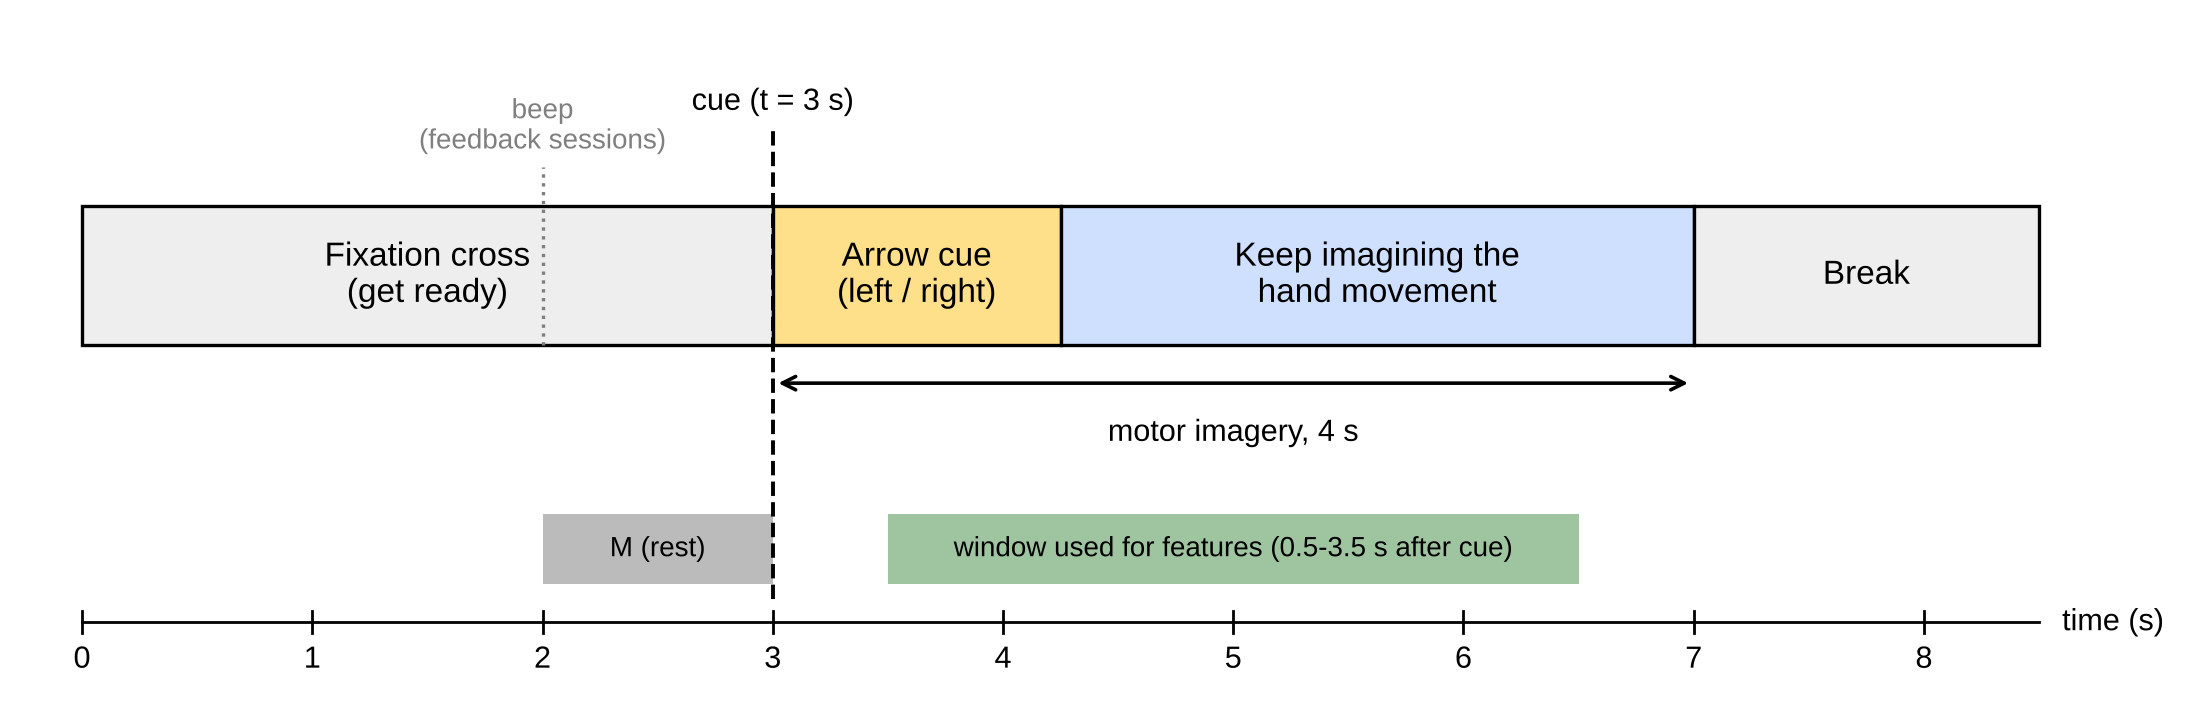
\includegraphics[width=\linewidth]{bci2b_trial_timing.png}
    \caption[Timing of one trial in the BCI Competition IV 2b dataset]%
            {Timing of one trial in the BCI Competition IV 2b dataset. $M$ is the rest
             period used as the reference for ERD/ERS, and the green bar is the window
             used for the classifier features}
    \label{fig:bci2b_timing}
\end{figure}

Figure~\ref{fig:bci2b_timing} shows what happens in one trial. A fixation cross appears at
the start, an arrow pointing left or right appears at 3 s, and the subject keeps imagining
the movement of that hand until about 7 s, after which there is a short break. One detail
in the files is easy to miss and cost a full round of work in this project. The position
stored for each trial is the start of the trial and not the moment of the cue, which comes
3 s later. The first classifiers trained here cut their windows from the trial start, so
they looked only at the fixation period and all of them came out at exactly chance level.
Once the windows were moved 3 s forward to the cue, the accuracies jumped to the values
reported below. The same kind of mistake, an event marker read in the wrong way, is
something to check first whenever a classifier gives exactly 50 per cent.

Only C3 and C4 were used for the ERD/ERS and PSD analysis, since those are the two motor
cortex channels the GELO headset has. The classifiers were run with all three channels and
again with only C3 and C4, and leaving out Cz lowered the cross-subject accuracy by less
than half a percentage point. Trials flagged as artefacts were kept in the main analysis.
The classifiers were also re-run with these trials removed, and the result changed by less
than half a percentage point, so the choice does not affect any conclusion.

\begin{figure}[!htbp]
    \centering
    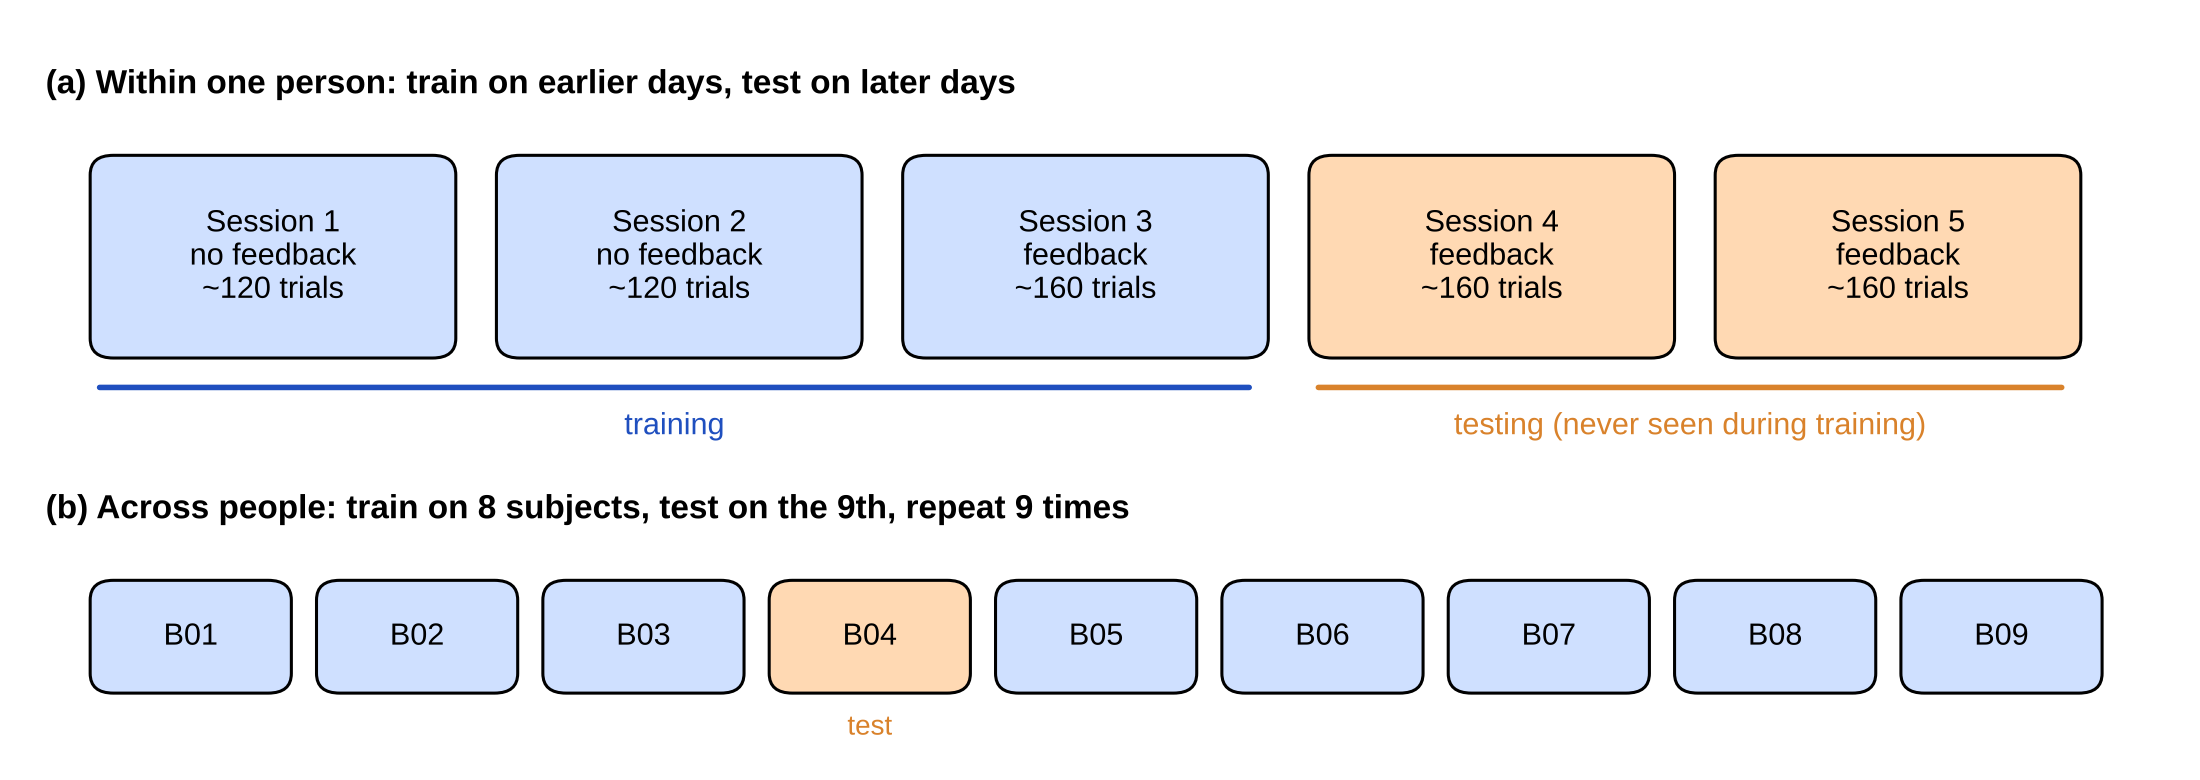
\includegraphics[width=\linewidth]{bci2b_data_split.png}
    \caption{The two ways the classifiers were tested on the BCI Competition IV 2b data}
    \label{fig:bci2b_split}
\end{figure}

Two ways of testing were used, as shown in Figure~\ref{fig:bci2b_split}. In the first, a
separate model is trained for each person on sessions 1 to 3 and tested on sessions 4 and
5, which were recorded on later days. This is the official split of the competition. In
the second, the model is trained on eight people and tested on the ninth, and this is
repeated so that every person is tested once. The second test is the one that matters most
for this project, because it shows whether a model can work on a new person with no
training data from that person, which is what the GELO headset would need. In both cases
the test trials are never used for training, for scaling the features or for choosing any
setting. The complete processing chain is shown in Figure~\ref{fig:bci2b_processing}.

\begin{figure}[!htbp]
    \centering
    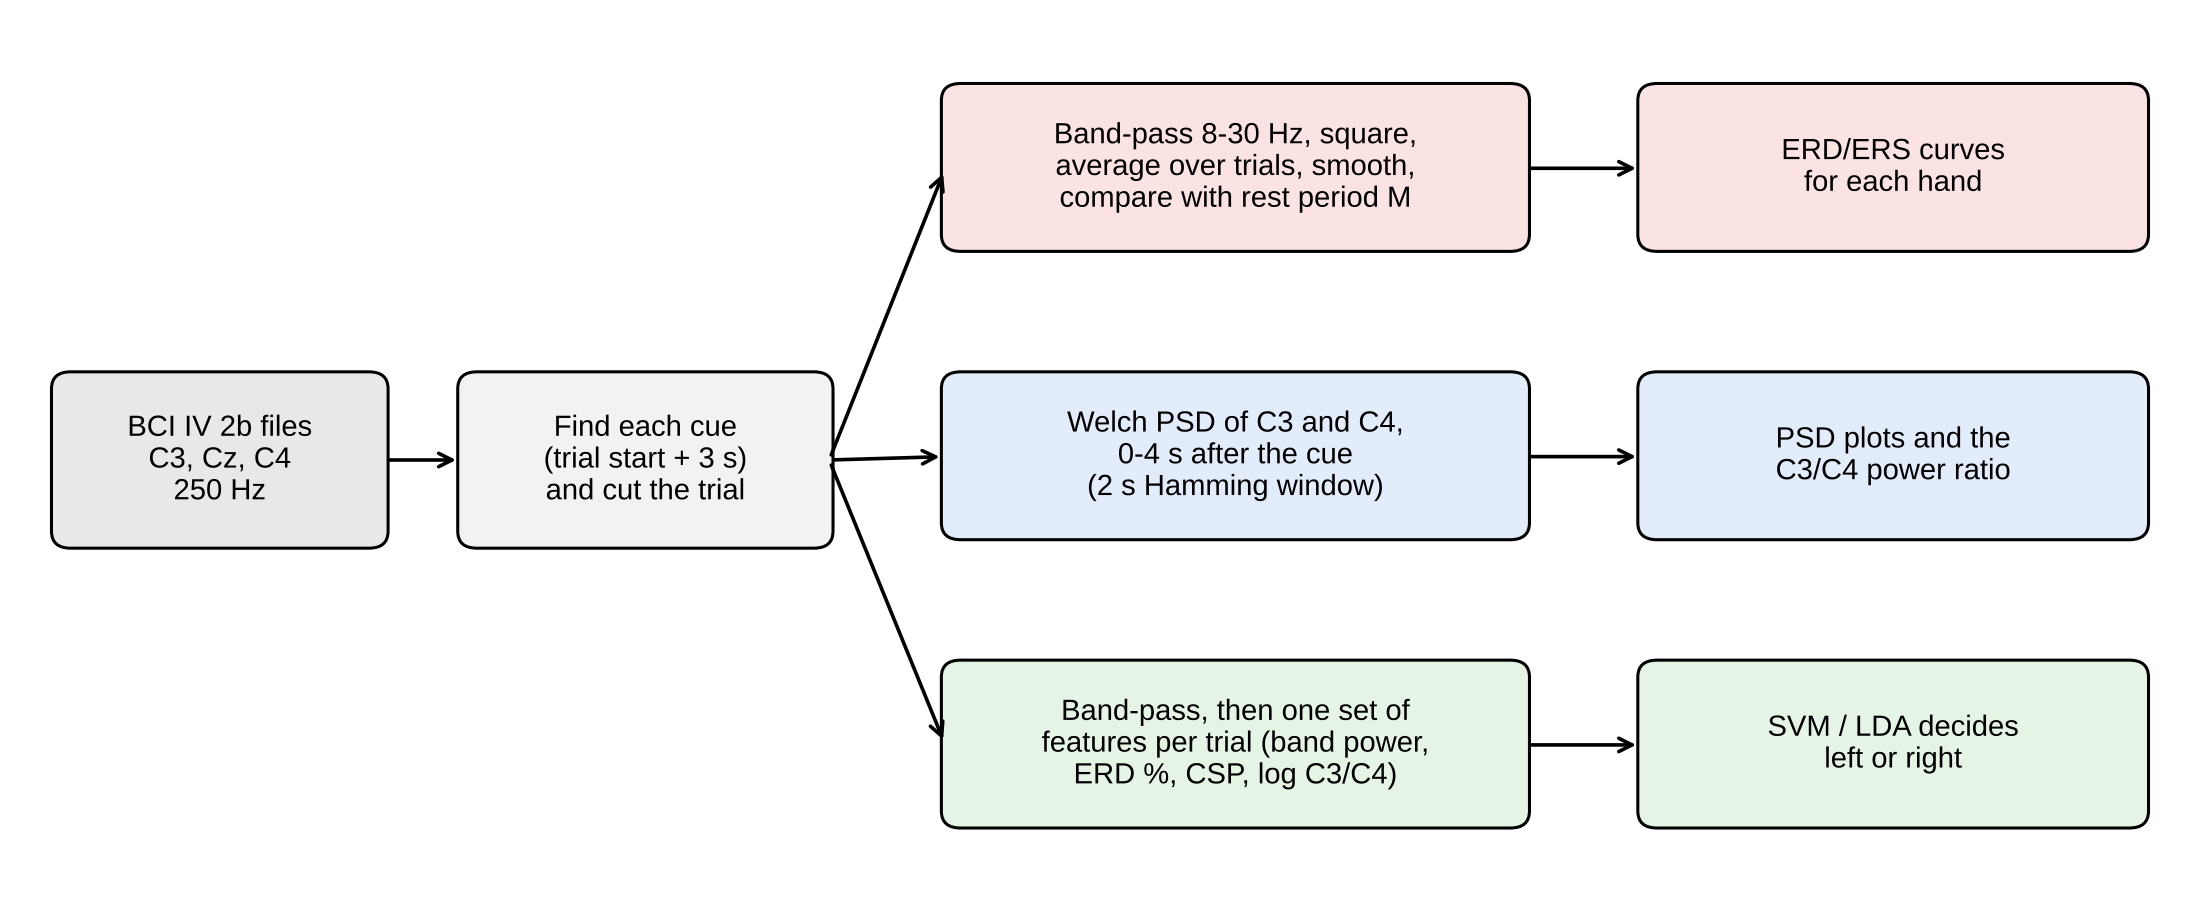
\includegraphics[width=\linewidth]{bci2b_processing.png}
    \caption{Processing chain used for the BCI Competition IV 2b data}
    \label{fig:bci2b_processing}
\end{figure}

\FloatBarrier

\subsection{ERD/ERS of the BCI Competition IV 2b Subjects}

The ERD/ERS was computed in exactly the same way as for the stroke patients. C3 and C4
were filtered between 8 and 30 Hz with a second-order zero-phase Butterworth filter,
squared to give power, averaged over all trials of the same hand, smoothed with a
100-sample moving average (0.4 s), and converted to a percentage change using the same
equation as before, with $M$ taken as the average power in the one second just before the
cue. Two small changes were made so that the whole trial can be seen. The plot covers the
full 8 s of the trial with the cue marked, and the filter was run on the trial with an
extra half second on each side, which was then cut off, so that the start and end of the
curve are not distorted by the filter.

\begin{figure}[!htbp]
    \centering
    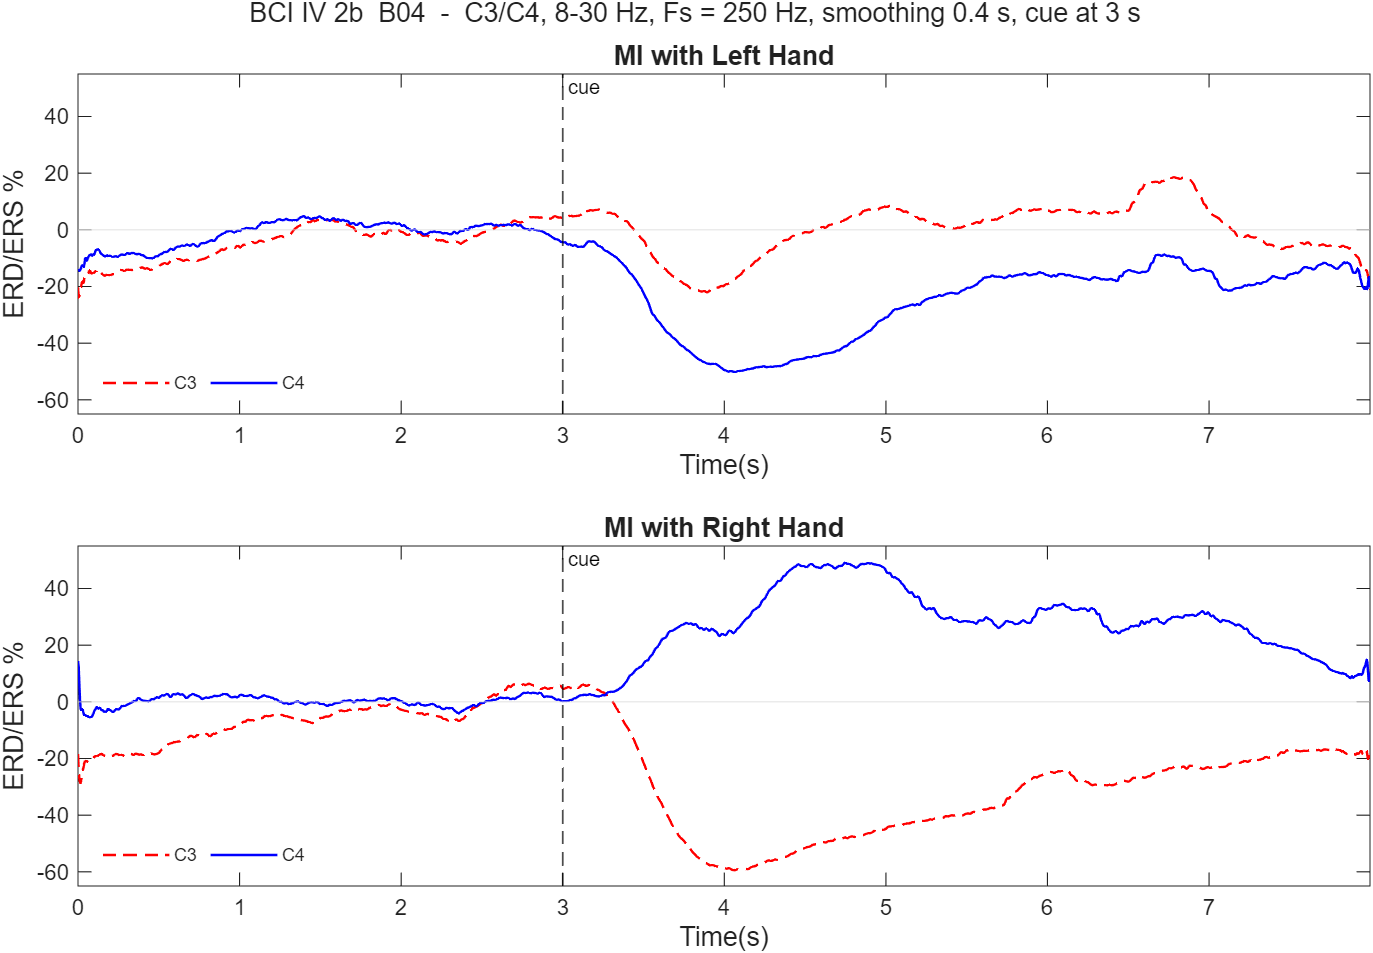
\includegraphics[width=0.95\linewidth]{bci2b_B04_erd.png}
    \caption[ERD/ERS of C3 and C4 for subject B04 of the BCI Competition IV 2b dataset]%
            {ERD/ERS of C3 and C4 for subject B04 of the BCI Competition IV 2b dataset,
             8--30 Hz, $F_s = 250$ Hz, 370 trials for each hand. The dashed line marks the
             cue at 3 s}
    \label{fig:bci2b_erd_b04}
\end{figure}

Figure~\ref{fig:bci2b_erd_b04} shows the result for subject B04, the subject with the
clearest pattern in the dataset. Before the cue both channels stay close to zero, as they
should, since nothing has happened yet. During left-hand imagery, C4 falls to about
$-50$ per cent within one second of the cue and stays well below C3 for the rest of the
imagery period, while C3 dips briefly and then returns close to the baseline. During
right-hand imagery the picture is reversed: C3 falls to about $-60$ per cent, and C4 not
only stays up but rises to about $+45$ per cent. This is the textbook pattern described in
Chapter 2~\cite{pfurtscheller1999erd}: imagining one hand lowers the 8--30 Hz power over the
opposite side of the head, and the side that is not involved can even become more
synchronised than at rest.

\begin{table}[!htbp]
\centering
\caption{Mean ERD/ERS (\%) from 0.5 to 3.5 s after the cue for every BCI Competition IV 2b subject}
\label{tab:bci2b_erd}
\begin{tabular}{|c|c|c|c|c|}
\hline
\multirow{2}{*}{\textbf{Subject}} & \multicolumn{2}{c|}{\textbf{Left-hand imagery}} & \multicolumn{2}{c|}{\textbf{Right-hand imagery}} \\
\cline{2-5}
 & \textbf{C3} & \textbf{C4} & \textbf{C3} & \textbf{C4} \\
\hline
B01 & $-15.4$ & $\mathbf{-40.0}$ & $\mathbf{-24.3}$ & $-15.7$ \\
B02 & $-13.7$ & $\mathbf{-31.8}$ & $-17.1$ & $-23.4$ \\
B03 & $-14.5$ & $\mathbf{-25.3}$ & $\mathbf{-20.4}$ & $-17.3$ \\
B04 & $-1.2$  & $\mathbf{-31.1}$ & $\mathbf{-42.2}$ & $+33.8$ \\
B05 & $-27.6$ & $\mathbf{-30.3}$ & $\mathbf{-35.1}$ & $-16.2$ \\
B06 & $-10.1$ & $\mathbf{-30.9}$ & $\mathbf{-29.9}$ & $-16.6$ \\
B07 & $-2.4$  & $\mathbf{-17.0}$ & $\mathbf{-27.8}$ & $+6.7$ \\
B08 & $-7.7$  & $\mathbf{-23.8}$ & $\mathbf{-37.6}$ & $+52.2$ \\
B09 & $-18.7$ & $-16.2$ & $\mathbf{-45.6}$ & $-2.6$ \\
\hline
Median & $-13.7$ & $-30.3$ & $-29.9$ & $-15.7$ \\
\hline
\end{tabular}
\end{table}

Table~\ref{tab:bci2b_erd} gives the average change for all nine subjects. The value in
bold is the channel opposite to the imagined hand whenever that channel dropped more. This
happens in 16 of the 18 cases. The two exceptions are B02 during right-hand imagery and
B09 during left-hand imagery, and in both of them the two channels dropped by similar
amounts rather than the wrong channel dropping clearly. The plots for all nine subjects
are collected in Figure~\ref{fig:bci2b_erd_all}.

\begin{figure}[!htbp]
    \centering
    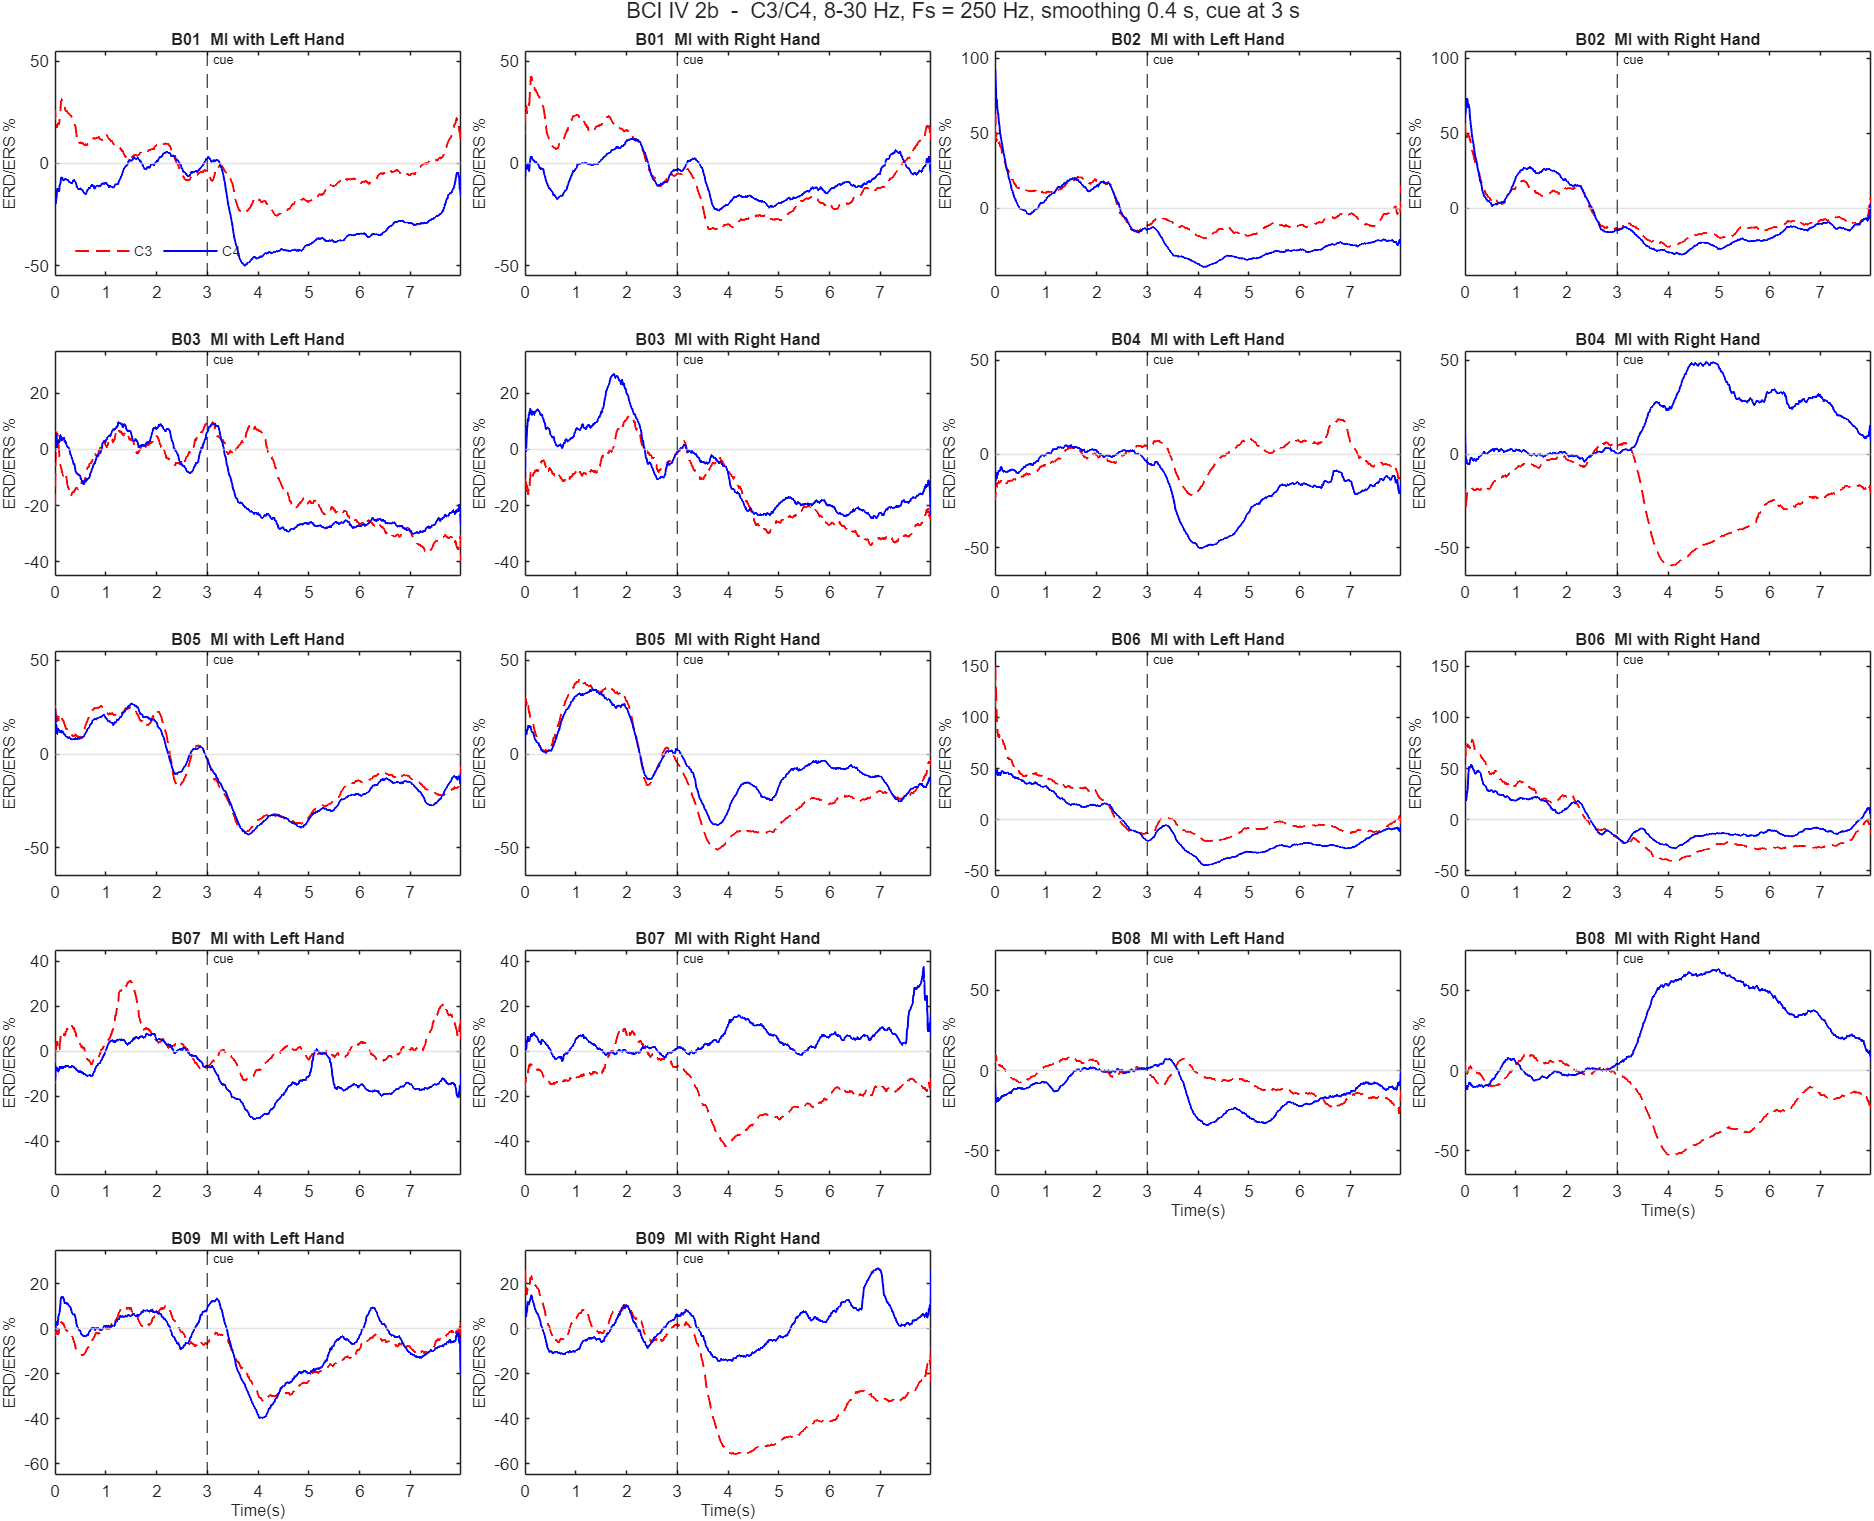
\includegraphics[width=\linewidth]{bci2b_erd_all.png}
    \caption{ERD/ERS of C3 and C4 for all nine subjects of the BCI Competition IV 2b dataset}
    \label{fig:bci2b_erd_all}
\end{figure}

There is one clear difference from the data recorded with the GELO headset. In BCI
Competition IV 2b both channels fall below the baseline after the cue, which is a true
desynchronisation, while in the recorded data both channels mostly rose. In 2b the second
before the cue is a calm fixation period, so $M$ is a real rest level. This supports the
explanation given later in Section~\ref{sec:recorded_results} that the baseline in the
recorded sessions is not a true rest period.

\FloatBarrier

\subsection{Power Spectral Density of Subject B04}

The PSD was computed with Welch's method~\cite{welch1967} on C3 and C4 for the 4 s after
the cue, using 2 s Hamming windows with 50 per cent overlap, which gives a resolution of
0.5 Hz. The spectra of all trials of the same hand were averaged. The C3/C4 ratio printed
above each figure is the power between 8 and 30 Hz at C3 divided by the power in the same
band at C4. Figures~\ref{fig:bci2b_psd_left} and~\ref{fig:bci2b_psd_right} use the same
layout as the PSD figures of the recorded data in Section~\ref{sec:recorded_results}, with
the two channels on top and the overlay below.

\begin{figure}[!htbp]
    \centering
    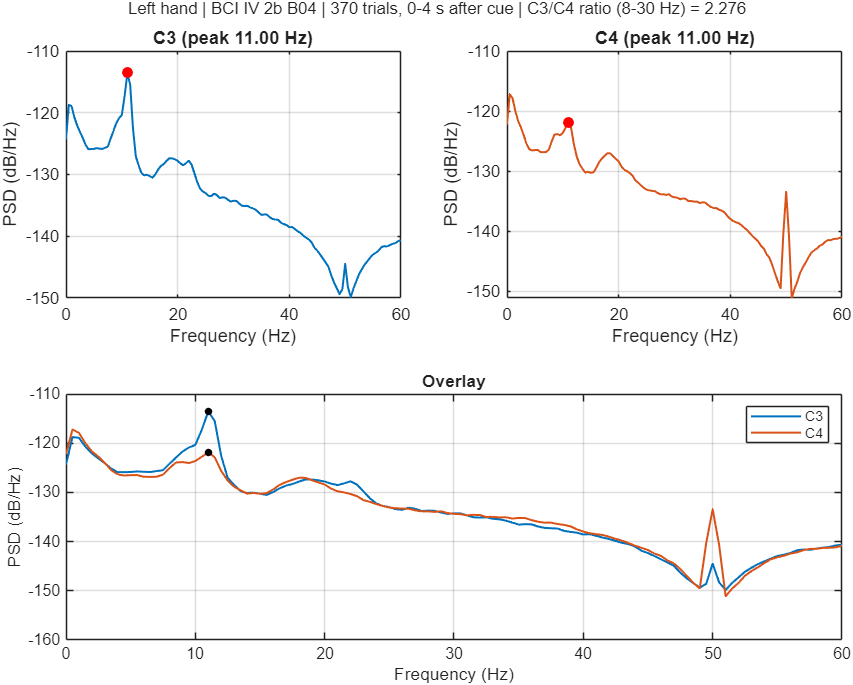
\includegraphics[width=0.85\linewidth]{bci2b_B04_psd_left.png}
    \caption{Power spectral density of C3 and C4 for imagined left-hand movement, subject B04
             of the BCI Competition IV 2b dataset}
    \label{fig:bci2b_psd_left}
\end{figure}

\begin{figure}[!htbp]
    \centering
    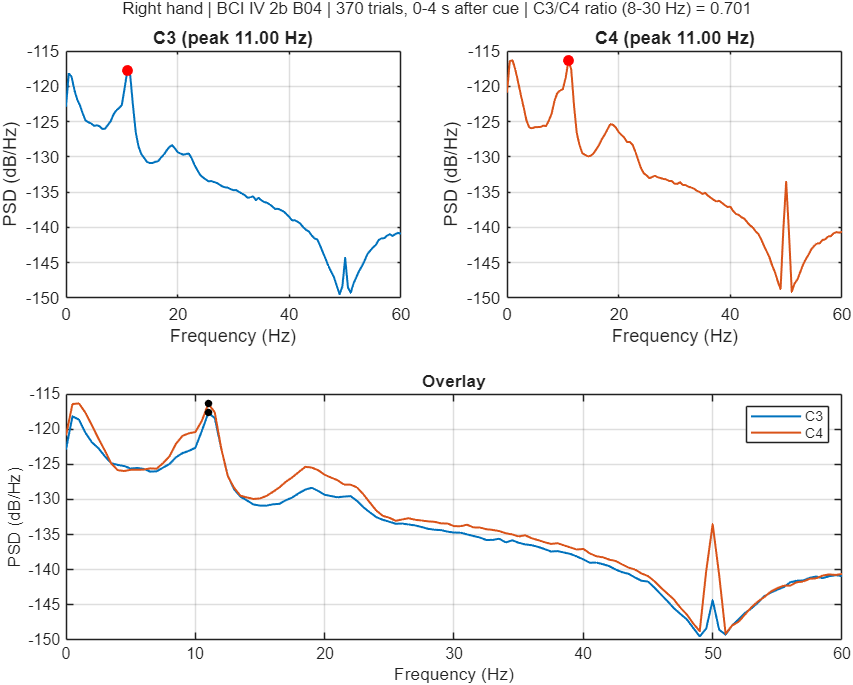
\includegraphics[width=0.85\linewidth]{bci2b_B04_psd_right.png}
    \caption{Power spectral density of C3 and C4 for imagined right-hand movement, subject B04
             of the BCI Competition IV 2b dataset}
    \label{fig:bci2b_psd_right}
\end{figure}

\FloatBarrier

Both channels have a clear peak at 11 Hz for both hands, which is the mu rhythm of the
motor cortex, and a smaller bump around 18 to 22 Hz in the beta band. The peak frequency
is the same in all four plots, so, just as with the recorded data, the peak frequency does
not tell the two hands apart. What changes is which channel is stronger. During left-hand
imagery the C3 peak stands about 8 dB above the C4 peak, because the power at C4, over the
right side of the head, has dropped. During right-hand imagery the order flips and C4 is
slightly above C3 across the mu and beta bands. As a result the C3/C4 ratio is 2.28 for
the left hand and 0.70 for the right hand. The sharp feature at 50 Hz comes from mains
interference and the notch filter used during recording, and it lies well outside the
8--30 Hz band used in this work.

\subsection{The C3/C4 Power Ratio as a Left and Right Detector}

The same ratio was computed for every subject, and the result is given in
Table~\ref{tab:bci2b_ratio} and Figure~\ref{fig:bci2b_ratio}. The reasoning behind it is
simple. Imagining the left hand lowers the power at C4, so C3/C4 goes up. Imagining the
right hand lowers the power at C3, so C3/C4 goes down. Using C4/C3 instead carries exactly
the same information, with the direction reversed.

\begin{table}[!htbp]
\centering
\caption{C3/C4 power ratio (8--30 Hz, 0--4 s after the cue) and single-trial accuracy of the ratio for each BCI Competition IV 2b subject}
\label{tab:bci2b_ratio}
\begin{tabular}{|c|c|c|c|c|}
\hline
\textbf{Subject} & \textbf{Left hand} & \textbf{Right hand} & \textbf{Left higher?} & \textbf{Accuracy, sessions 4--5} \\
\hline
B01 & 0.96 & 0.63 & Yes & 60.9\% \\
B02 & 0.91 & 0.83 & Yes & 55.7\% \\
B03 & 1.21 & 1.08 & Yes & 56.3\% \\
B04 & \textbf{2.28} & \textbf{0.70} & Yes & \textbf{96.6\%} \\
B05 & 0.98 & 0.71 & Yes & 69.1\% \\
B06 & 1.30 & 0.87 & Yes & 79.1\% \\
B07 & 1.14 & 0.80 & Yes & 69.4\% \\
B08 & 0.92 & 0.31 & Yes & 90.6\% \\
B09 & 1.05 & 0.58 & Yes & 83.8\% \\
\hline
Mean & & & 9 of 9 & 73.5\% \\
\hline
\end{tabular}
\end{table}

\begin{figure}[!htbp]
    \centering
    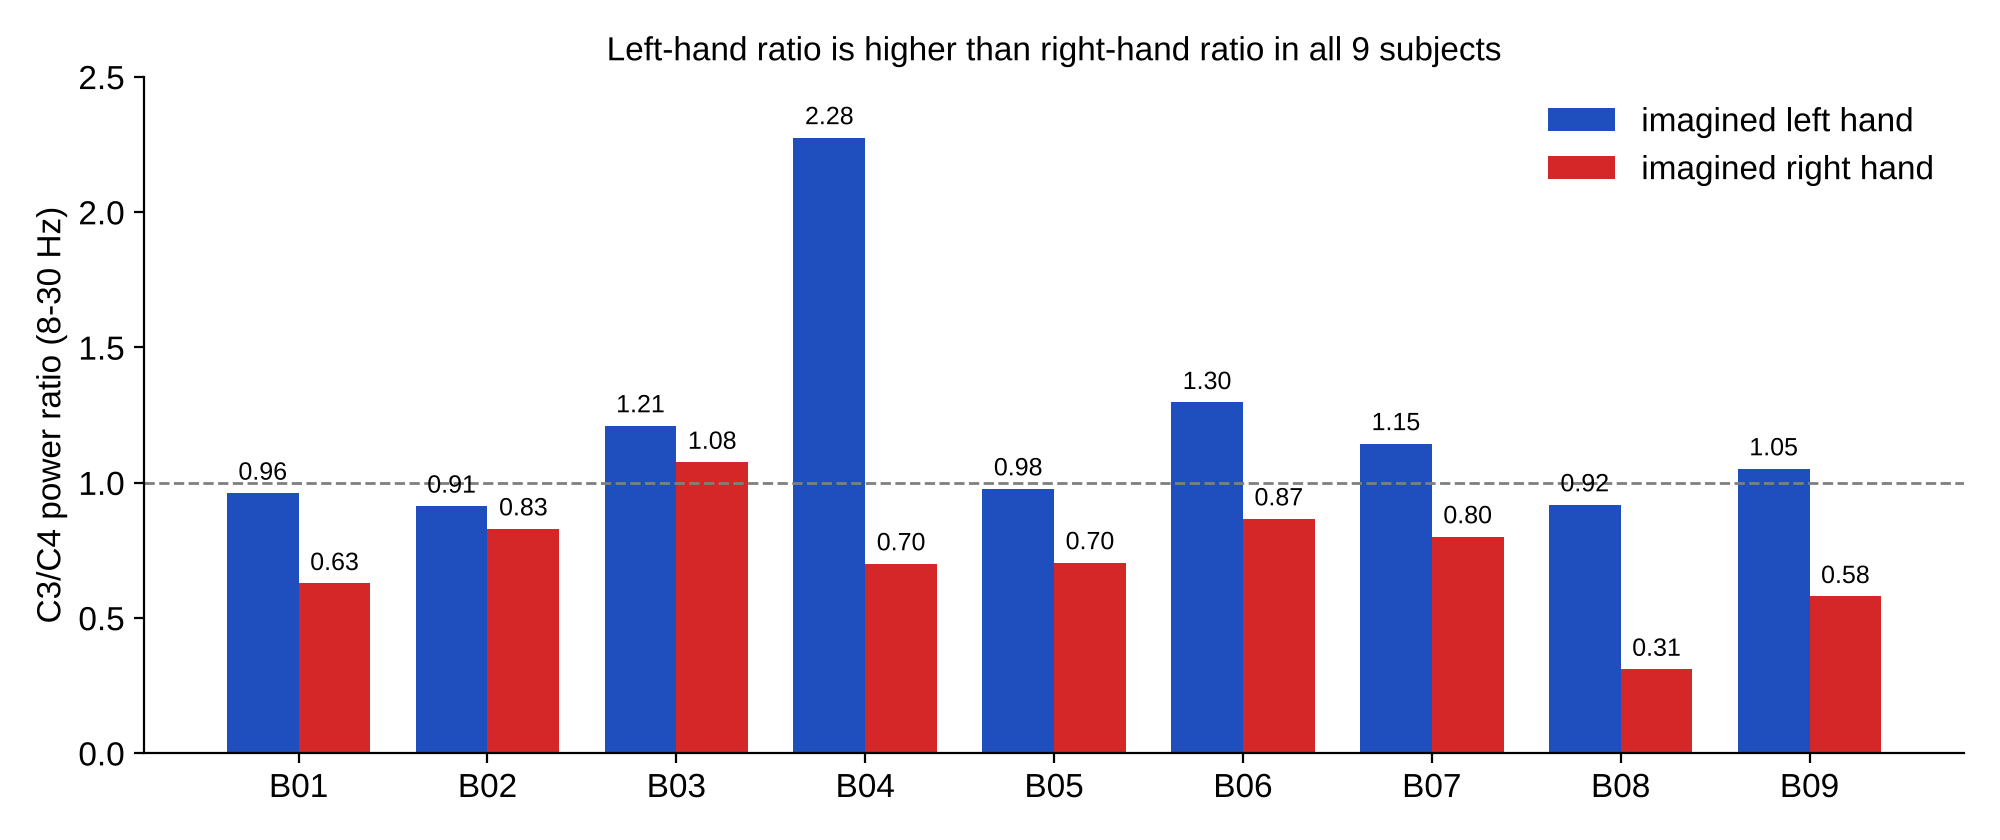
\includegraphics[width=0.95\linewidth]{bci2b_ratio_bars.png}
    \caption{C3/C4 power ratio for imagined left and right hand in each BCI Competition IV 2b subject}
    \label{fig:bci2b_ratio}
\end{figure}

For every one of the nine subjects the ratio is higher for the left hand than for the
right hand. The figure also shows something important for using the ratio in practice:
the value itself changes from person to person. For B03 both values are above 1, and for
B08 both are below 1. A fixed rule such as ``left if the ratio is above 1'' would
therefore fail for some people, and the dividing line has to be learned for each person,
or the data has to be brought to a common scale first.

To check whether the ratio works on single trials and not only on averages, one number was
computed per trial, the logarithm of the C3/C4 power ratio in the 8--30 Hz band from 0.5 to
3.5 s after the cue. A single threshold was learned from each subject's sessions 1 to 3
and then applied, unchanged, to sessions 4 and 5. The same test was done for the other
simple single-number features: the power of each channel on its own, the ERD of each
channel on its own, and the difference between the ERD of C3 and C4. The results are
shown in Figure~\ref{fig:bci2b_single}.

\begin{figure}[!htbp]
    \centering
    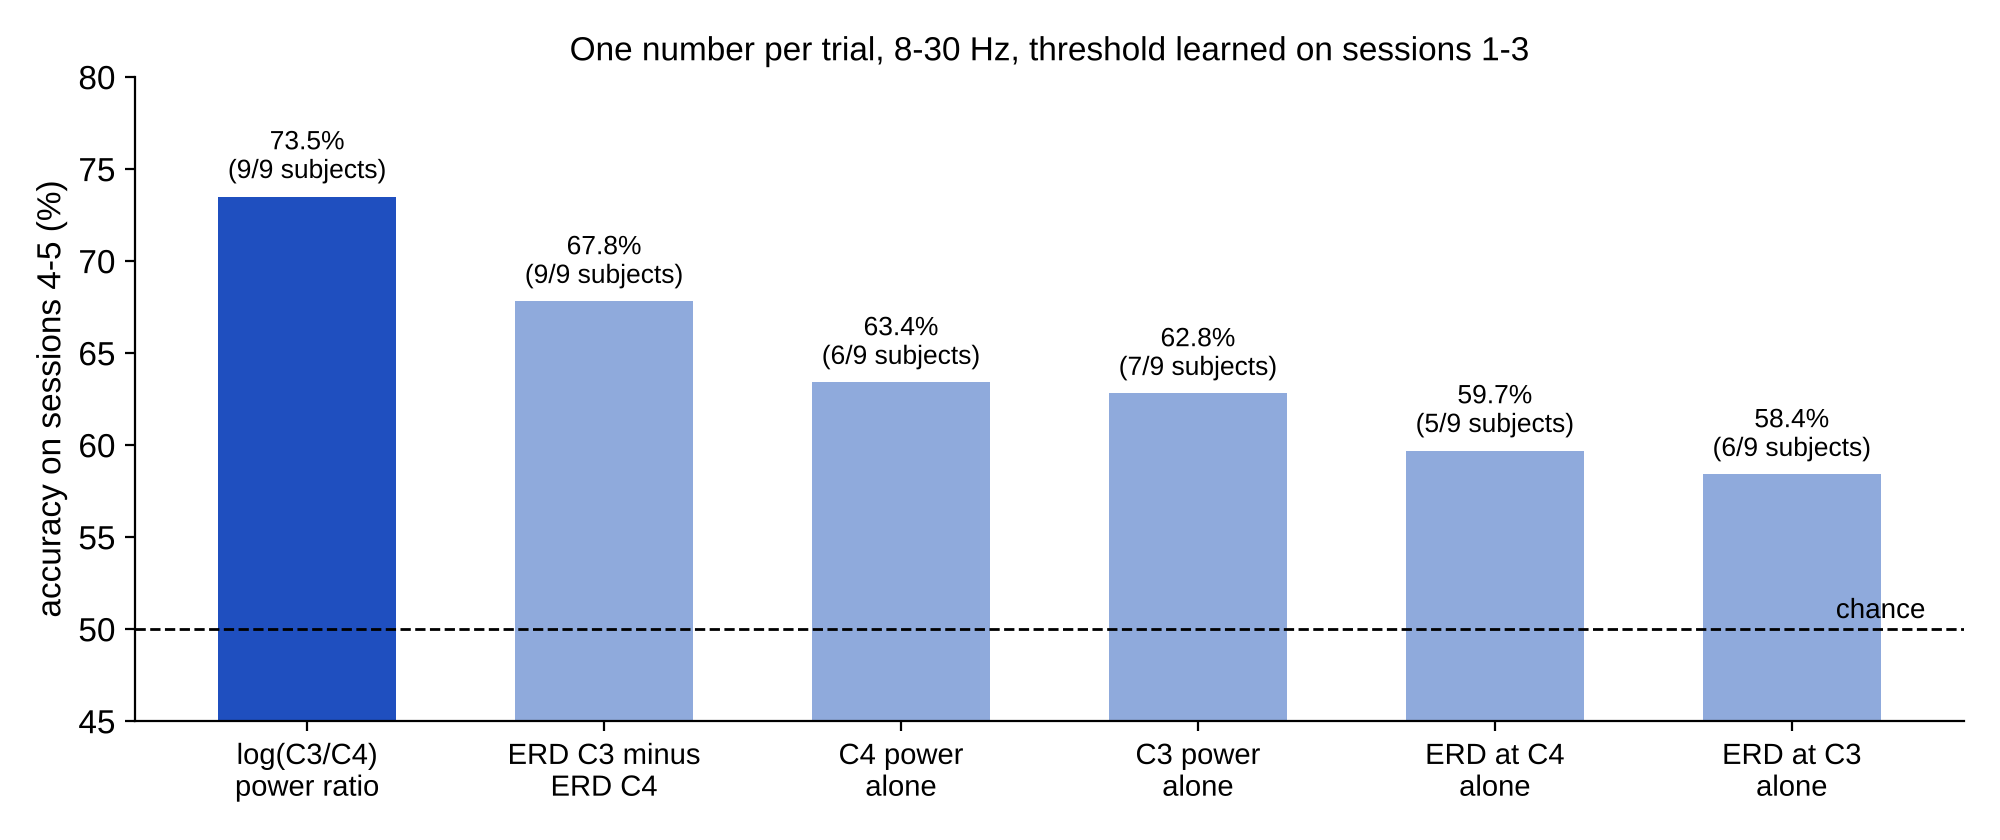
\includegraphics[width=0.95\linewidth]{bci2b_single_feature.png}
    \caption[Single-trial accuracy of one-number features on the BCI Competition IV 2b dataset]%
            {Single-trial accuracy of one-number features on sessions 4 and 5 of the BCI
             Competition IV 2b dataset, mean of nine subjects. The count under each value
             is the number of subjects for whom the feature was better than chance
             (binomial test, $p < 0.05$)}
    \label{fig:bci2b_single}
\end{figure}

The log C3/C4 ratio is the best single number by a clear margin. It reaches 73.5 per cent
on average on days the threshold never saw, from 55.7 per cent for B02 to 96.6 per cent
for B04, and it is better than chance for all nine subjects. When the threshold was
learned from eight other people instead of from the subject's own sessions, it still
reached 70.8 per cent. The power of either channel on its own reaches only about 63 per
cent, and the ERD of either channel on its own about 58 to 60 per cent. There are two
reasons why the ratio does so much better. First, anything that makes both channels
stronger or weaker together, such as a change in electrode contact, amplifier gain or how
alert the person is on that day, cancels out when one channel is divided by the other.
Second, the ratio does not need a baseline period at all, while ERD does, and an
unreliable baseline was exactly the problem seen in the recorded data. This is the
strongest evidence in this work that the C3/C4 ratio is a sound feature for telling left
from right, and it supports the decision to include it in the SVM feature sets used on the
recorded data.

\FloatBarrier

\subsection{SVM Training and Classification Accuracy}

Several classifiers were trained on the BCI Competition IV 2b data, starting with an SVM
on ERD features, which is the closest to what was done for the stroke patients, and then
moving to the standard motor imagery methods.

\textbf{ERD\% with an SVM.} For each trial, the ERD\% at C3, Cz and C4 was computed in the mu
band (8--13 Hz) and the beta band (13--30 Hz), giving six features. The rest period was
taken from 2 to 1 s before the cue, so that it ends before the warning beep, and the task
period from 0.5 to 3.5 s after the cue. Linear and radial basis function SVMs were trained
with the MATLAB function \texttt{fitcsvm} on standardised features, on sessions 1 to 3, and
tested on sessions 4 and 5. Since the ERD curves earlier in this chapter are averages over
many trials, the same idea was also tried for the classifier: power was averaged over a
group of 5 or 10 trials of the same hand before the ERD was computed. The groups were
formed separately inside the training data and inside the test data, so no trial is ever
shared between them. The results are given in Table~\ref{tab:bci2b_erdsvm}.

\begin{table}[!htbp]
\centering
\caption{Accuracy of the ERD\% SVM on sessions 4 and 5 of the BCI Competition IV 2b dataset, mean of nine subjects}
\label{tab:bci2b_erdsvm}
\begin{tabular}{|l|c|c|}
\hline
\textbf{Trials averaged for one decision} & \textbf{Linear kernel} & \textbf{RBF kernel} \\
\hline
1 (single trial) & 65.9\% & 57.8\% \\
\hline
5 & 77.9\% & 75.6\% \\
\hline
10 & 80.6\% & 79.4\% \\
\hline
\end{tabular}
\end{table}

On single trials the linear SVM reaches 65.9 per cent, which is already well above the 50
to 54 per cent obtained when the models were trained on the stroke data and tested on the
recorded data (Table~\ref{tab:svm_accuracy}). Averaging trials helps a great deal, raising
the accuracy to 80.6 per cent for groups of ten. The price is that one decision then needs
ten trials of the same hand, so this is useful for a slow, reliable command but not for
fast control. The linear kernel is better than the RBF kernel in every case, which is
expected with so few features and so much variation between days. When the same ERD\% SVM
was trained on eight subjects and tested on the ninth, it reached 62.0 per cent on single
trials and 74.4 per cent with ten-trial averaging.

\textbf{Standard motor imagery classifiers.} The covariance-based methods described in
Chapter 2 were then trained in Python with scikit-learn~\cite{pedregosa2011sklearn}, all on
the 8--30 Hz band and the 0.5 to 3.5 s window after the cue. These were log band power of
the three channels with a linear SVM, CSP~\cite{ramoser2000csp} with LDA and with an SVM,
filter bank CSP~\cite{ang2012fbcsp} with an SVM, and a Riemannian tangent space
method~\cite{barachant2012riemann} with an SVM. The SVM settings were chosen by
cross-validation inside the training data only. Each model was run with and without
Euclidean alignment~\cite{he2020ea}. Euclidean alignment re-centres the data of each
session using the average covariance of that session, so that differences in overall
signal size and channel correlation between days or between people are removed before
training. It uses no labels, so it can also be applied to the test session without
leaking any information. The results for both ways of testing are given in
Table~\ref{tab:bci2b_models}.

\begin{table}[!htbp]
\centering
\caption{Classification accuracy on the BCI Competition IV 2b dataset, mean of nine subjects}
\label{tab:bci2b_models}
\begin{tabular}{|l|c|c|c|c|}
\hline
\multirow{2}{*}{\textbf{Model}} & \multicolumn{2}{c|}{\textbf{Same person, later days}} & \multicolumn{2}{c|}{\textbf{New person}} \\
\cline{2-5}
 & \textbf{Without EA} & \textbf{With EA} & \textbf{Without EA} & \textbf{With EA} \\
\hline
Log band power + SVM & 73.0\% & 78.5\% & 69.5\% & 74.7\% \\
\hline
CSP + LDA & 74.8\% & 79.1\% & 70.0\% & \textbf{74.7\%} \\
\hline
CSP + SVM & 74.8\% & 79.0\% & 70.4\% & 74.7\% \\
\hline
Filter bank CSP + SVM & 76.7\% & \textbf{80.2\%} & 69.4\% & 73.5\% \\
\hline
Tangent space + SVM & 75.5\% & 78.5\% & 69.2\% & 74.6\% \\
\hline
log(C3/C4) threshold only & \multicolumn{2}{c|}{73.5\%} & \multicolumn{2}{c|}{70.8\%} \\
\hline
\end{tabular}
\end{table}

The best result when a model is trained on the same person is 80.2 per cent, from filter
bank CSP with an SVM and Euclidean alignment. The best result on a person the model has
never seen is 74.7 per cent, and every one of the nine subjects is above chance in that
test. Three points stand out from the table. Euclidean alignment improved every single
model in both tests, by about 3 to 6 percentage points. The choice of model matters very
little: with alignment, all five models are within about 2 percentage points of each
other, and the simplest one, three log band powers with a linear SVM, ties for best on new
people. With only three channels, all of these methods end up reading the same small
amount of spatial information, so there is little room for a cleverer model to find
more. Finally, a single threshold on the C3/C4 ratio, with no SVM at all, is only about 4
to 7 percentage points behind the best models, which again shows how much of the useful
information that one number carries.

\begin{figure}[!htbp]
    \centering
    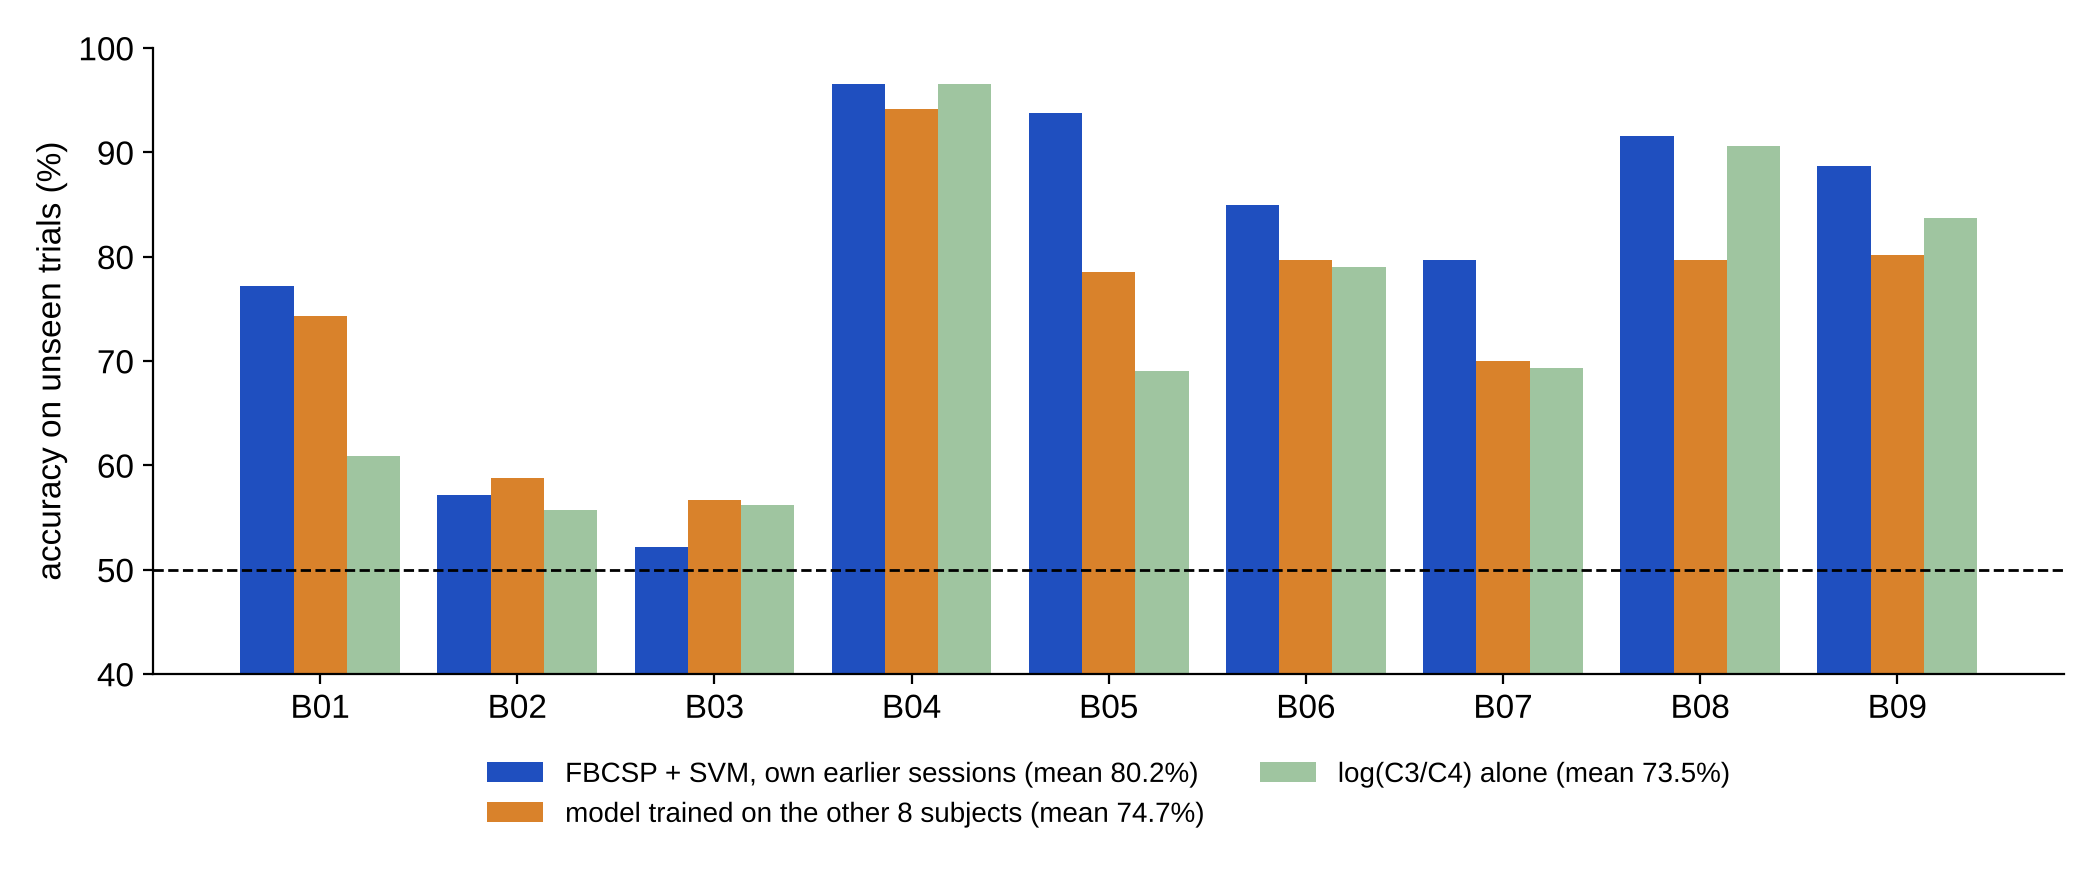
\includegraphics[width=\linewidth]{bci2b_accuracy_subjects.png}
    \caption{Accuracy for each BCI Competition IV 2b subject with the best model for each test and with the C3/C4 ratio alone}
    \label{fig:bci2b_subjects}
\end{figure}

Figure~\ref{fig:bci2b_subjects} shows the accuracy for each person. Subject B04 is the
best in every test, with 96.6 per cent when trained on its own earlier sessions, 94.2 per
cent from a model that never saw B04, and 96.6 per cent from the C3/C4 ratio alone. B05,
B08 and B09 are also close to or above 90 per cent with their own training data. At the
other end, B02 and B03 stay between 52 and 59 per cent whatever method is used. This is a
well-known effect in BCI research: a fraction of people do not produce a clear enough
motor imagery pattern for any current method to pick up, and no change of classifier
fixes it.

\begin{table}[!htbp]
\centering
\caption{Confusion matrix for the new-person test using only C3 and C4, all 6520 trials (CSP + SVM with Euclidean alignment)}
\label{tab:bci2b_confusion}
\begin{tabular}{|l|c|c|c|}
\hline
 & \textbf{Predicted left} & \textbf{Predicted right} & \textbf{Correct} \\
\hline
\textbf{True left}  & 2454 & 806  & 75.3\% \\
\hline
\textbf{True right} & 849  & 2411 & 74.0\% \\
\hline
\end{tabular}
\end{table}

Table~\ref{tab:bci2b_confusion} gives the confusion matrix for the new-person test using
only the two channels the GELO headset has, with every trial of every subject counted
once. The overall accuracy is 74.6 per cent, almost the same as with three channels, and
the errors are split almost evenly between the two hands. The model is not leaning
towards one class, which was a problem with the models trained on the stroke data.

\FloatBarrier

\subsection{Testing a BCI Competition IV 2b Model on the Recorded Data}

Since the 2b model works well on people it has never seen, the next question was whether
it works on the data recorded with the GELO headset. A model was trained on all nine 2b
subjects using only C3 and C4, with Euclidean alignment, and applied without any change
to the 72 usable recorded trials, cut with the same 0.5 to 3.5 s window after each marker.
Because each recorded file contains only one class, trials from the same file are not
independent, so the fair count is per file, giving 15 decisions.

The result was at chance. Across eight combinations of model and alignment, between 4 and
6 of the 15 files were classified correctly, and the best permutation test gave
$p = 0.83$, meaning a result this good is expected most of the time even with random
labels. The predictions were split roughly evenly between left and right, so the failure
is not a bias towards one class. To see why, the separation given by the log C3/C4 ratio
was measured directly on both datasets, using the area under the ROC curve, where 0.5
means no separation and values further from 0.5 mean better separation. For the 2b data
it was 0.22, a distance of 0.28 from 0.5. For the 72 recorded trials it was 0.51, a
distance of only 0.01. Taken over all recorded trials, the left and right difference in
the C3/C4 balance is therefore about twenty times weaker than in 2b, even though single
trials such as the one in Figure~\ref{fig:psd_left} show a large difference.

This is a useful negative result. The same code and the same model reach 74.6 per cent on
new people in 2b, so the classifier itself is working. What stands between it and the
GELO headset is the recorded data, most likely the way it was collected: each class was
recorded in separate files, markers were placed by hand, the baseline is not a true rest
period, and there are only 72 trials. The BCI Competition IV 2b protocol, with left and
right trials mixed within one session, fixed cue timing and several sessions per person,
is a direct model for how the next GELO recordings should be made.

\FloatBarrier

\section{Results on the Recorded Data}
\label{sec:recorded_results}

\subsection{ERD/ERS of the Recorded Data}

The same analysis was then applied to the data recorded with the GELO headset.
Figure~\ref{fig:erd_ours} shows the result for one subject over the four second imagination
window.

\begin{figure}[!htbp]
    \centering
    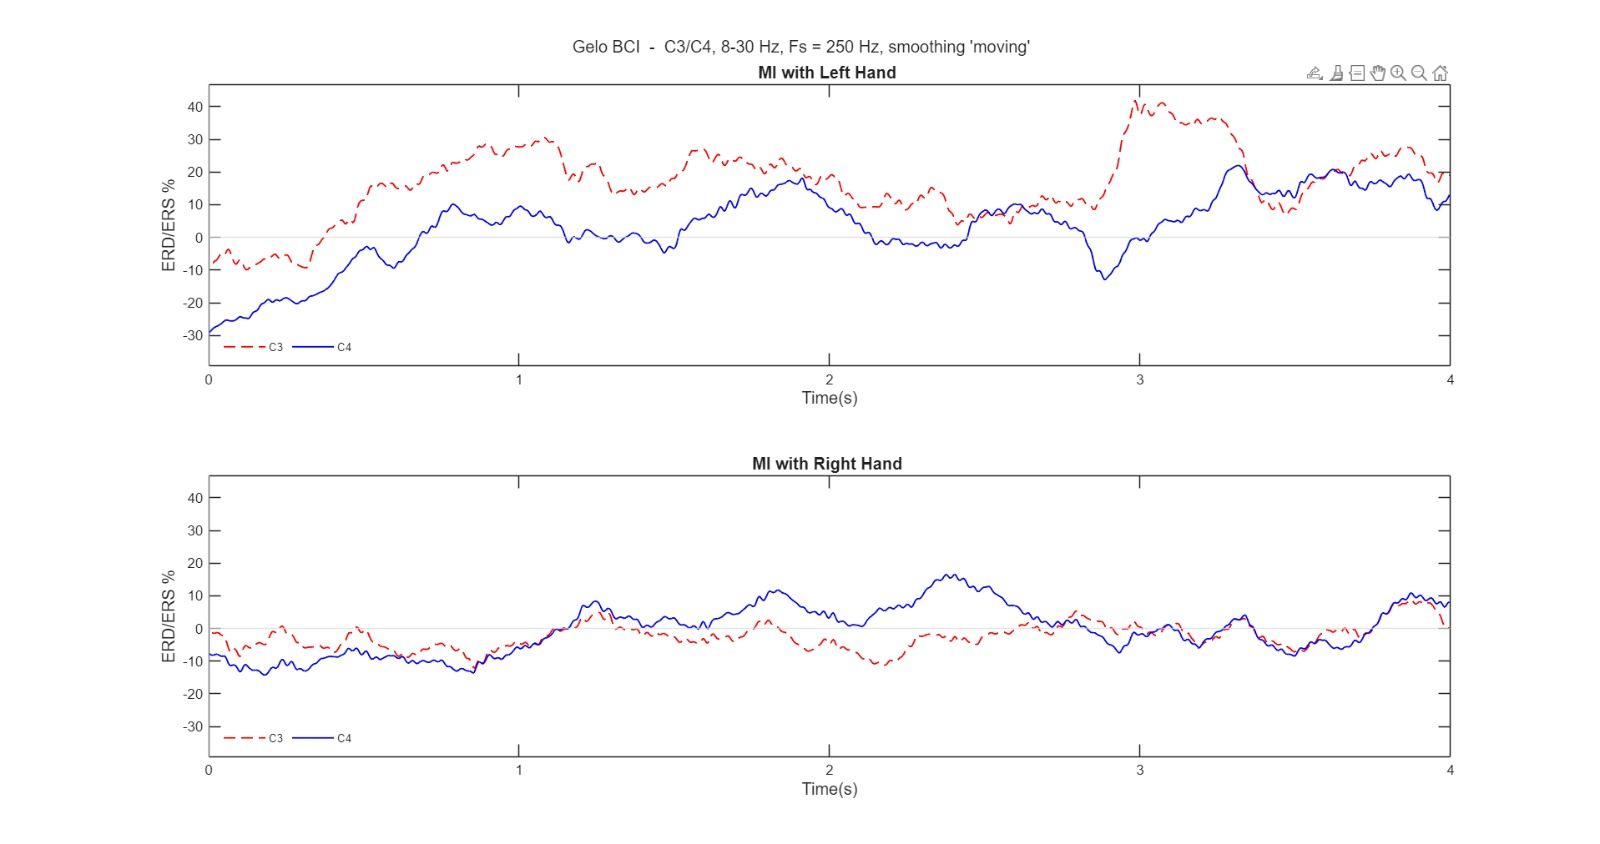
\includegraphics[width=0.95\linewidth]{erd_ours.jpg}
    \caption{ERD/ERS of C3 and C4 for the data recorded in this project, 8--30 Hz,
             $F_s = 250$ Hz}
    \label{fig:erd_ours}
\end{figure}

Two things can be seen from this figure. The first is that the two classes do separate. For
left-hand imagery the C3 trace stays above C4 for most of the window, reaching 20 to 40 per
cent, while for right-hand imagery the order reverses and C4 stays above C3, with both
traces remaining within roughly $\pm 15$ per cent. The sign of the difference between the
two channels therefore flips between the two classes, which is the property a classifier
can make use of.

The second is that the separation does not take the same form as in the reference dataset.
In the reference recording the contralateral channel falls below the baseline, giving a
clear desynchronisation, whereas in the recorded data both channels mostly rise above the
baseline and the difference between them is what carries the class information. There are
two likely reasons for this. The baseline period in the recorded sessions is taken from the
seconds immediately before the marker, during which the subject is already preparing for
the task, so the reference power is not a true rest level. In addition, the four-channel dry
headset picks up more muscle and movement artefact than the 30-channel saline system used
for the reference dataset, and these artefacts raise the power in the 8--30 Hz band. The
result is still usable, but it means the absolute ERD values from this setup should not be
compared directly against published values.

\FloatBarrier

\subsection{Power Spectral Density for Left and Right Imagery}

The PSD of the two motor cortex channels was computed for each trial.
Figure~\ref{fig:psd_left} shows a left-hand trial and Figure~\ref{fig:psd_right} a
right-hand trial from the same subject. In both figures the upper two plots show the two
channels separately and the lower plot overlays them, with the spectral peak marked.

\begin{figure}[!htbp]
    \centering
    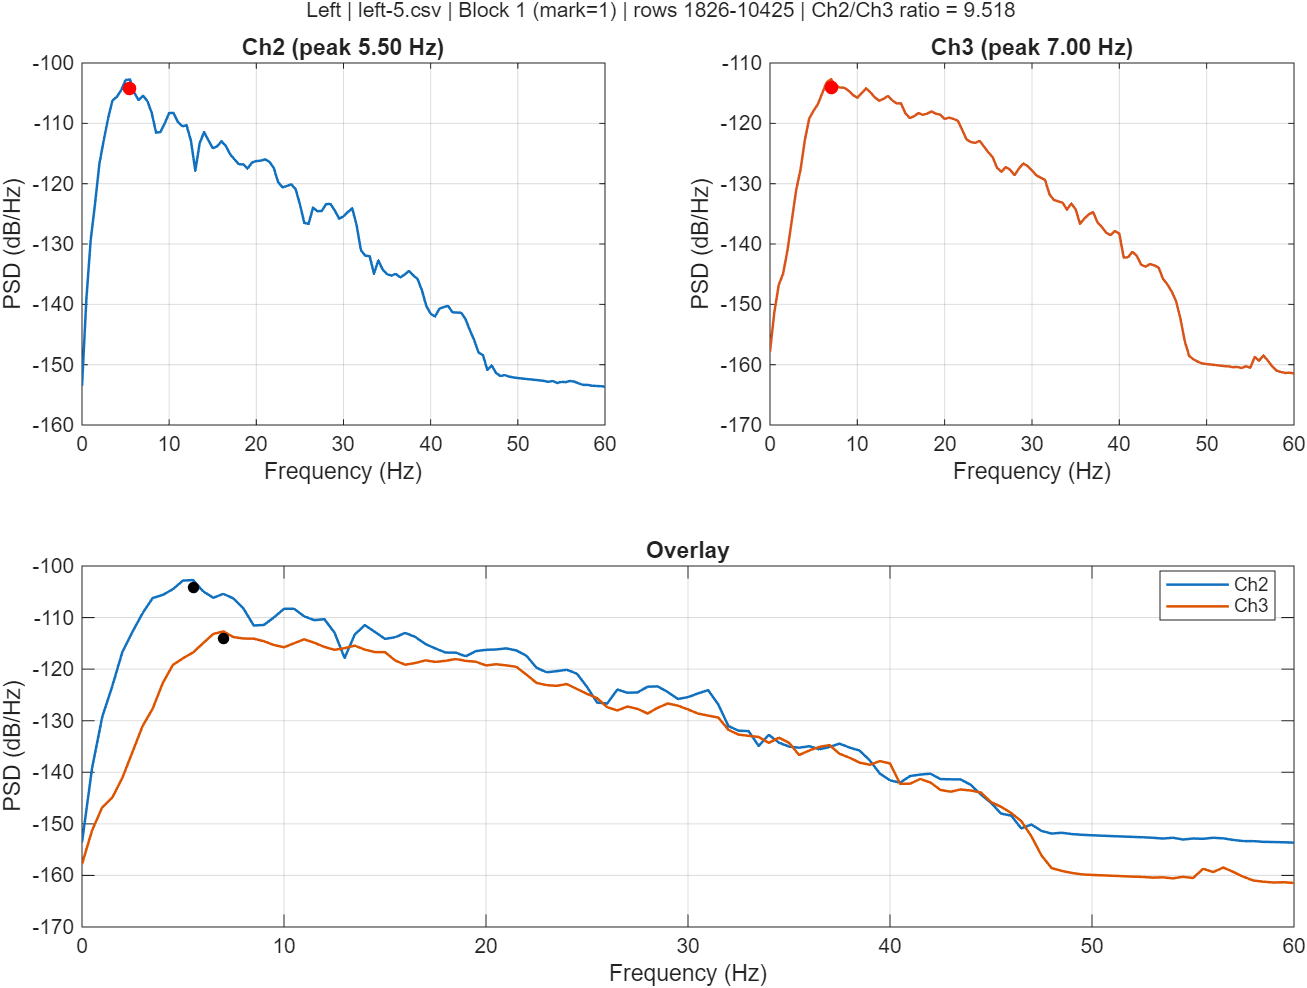
\includegraphics[width=0.85\linewidth]{psd_left_mi.png}
    \caption{Power spectral density of C3 and C4 for an imagined left-hand grasp}
    \label{fig:psd_left}
\end{figure}

\begin{figure}[!htbp]
    \centering
    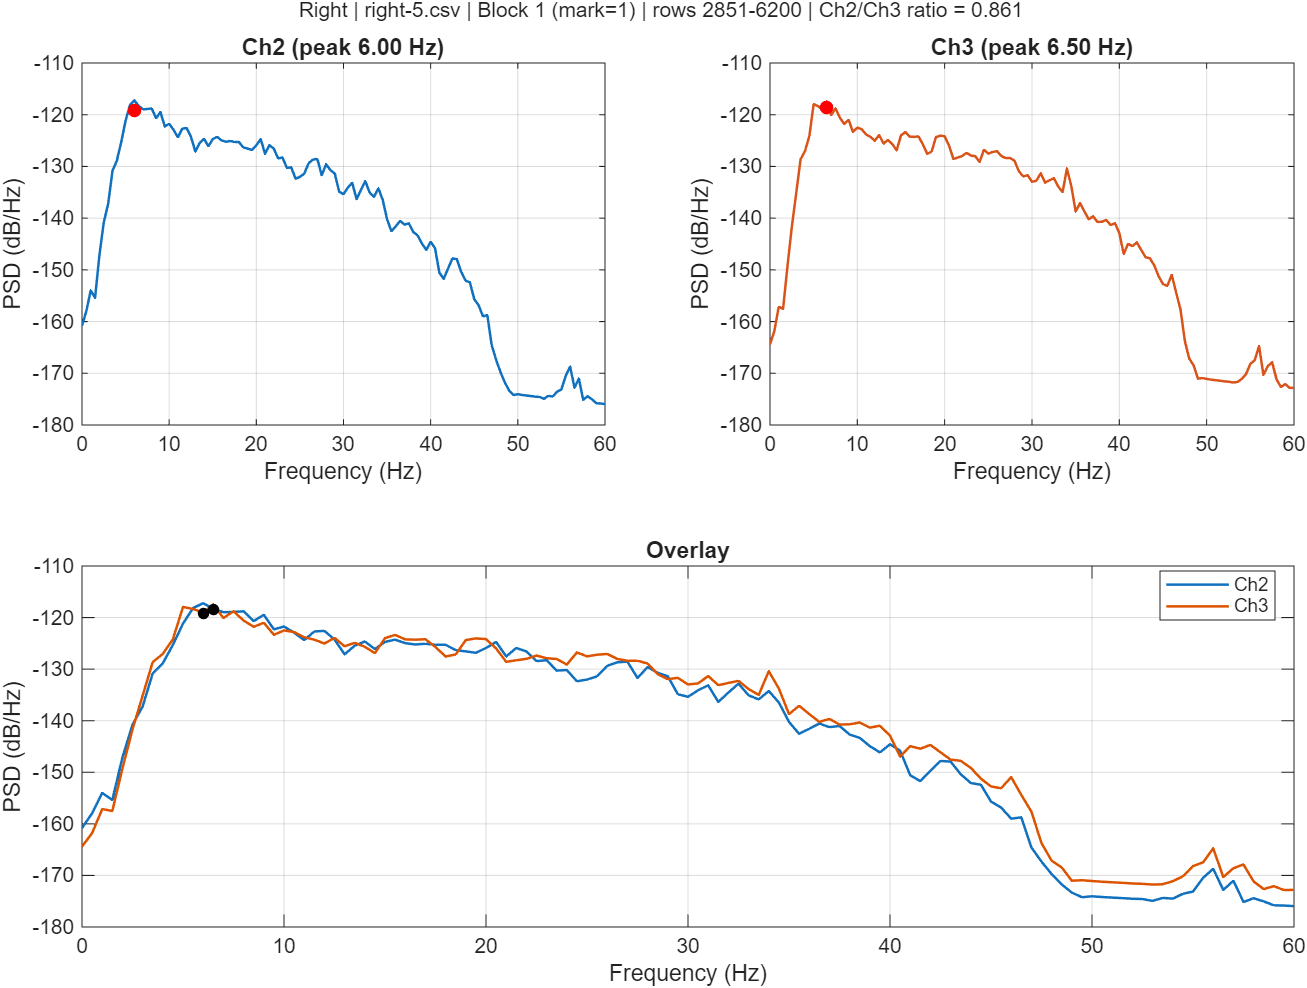
\includegraphics[width=0.85\linewidth]{psd_right_mi.png}
    \caption{Power spectral density of C3 and C4 for an imagined right-hand grasp}
    \label{fig:psd_right}
\end{figure}

\FloatBarrier

The difference between the two cases is clearest in the overlay plots. For the left-hand
trial the C3 curve sits roughly 10 dB above the C4 curve across most of the low frequency
range, giving a C3 to C4 power ratio of 9.52. For the right-hand trial the two curves lie
almost on top of each other, with a ratio of 0.86. The spectral peaks are close together in
both cases, at 5.50 Hz and 7.00 Hz for the left trial and 6.00 Hz and 6.50 Hz for the right
trial, which shows that the peak frequency itself does not separate the classes. It is the
balance of power between the two hemispheres, and not the shape of the spectrum, that
carries the useful information. This is the reason the logarithm of the C3 to C4 power
ratio was included as a feature for the classifier.

Both figures also show that the signal falls away sharply beyond about 45 Hz. This is the
effect of the filtering applied inside the device, and it is why the analysis in this work
is restricted to the 8--30 Hz range for motor imagery.

\FloatBarrier

\subsection{Classification Results}

Support Vector Machine classifiers were trained using the reference
dataset~\cite{liu2024mi} as training data and the data recorded in this project as test
data. Three feature sets were tried, each with both a linear and a radial basis function
kernel, and each using absolute power as well as ERD power:

\begin{itemize}
    \item \textbf{SVM-A:} mean, median, skewness and kurtosis of C3 and C4 (8 features)
    \item \textbf{SVM-B:} the above, plus $\log_{10}(P_{C3}/P_{C4})$ and the Welch band
          power over 8--30 Hz (9 features)
    \item \textbf{SVM-C:} the C3 to C4 power ratio alone (1 feature)
\end{itemize}

The accuracies obtained are summarised in Table~\ref{tab:svm_accuracy}.

\begin{table}[h]
\centering
\caption{Classification accuracy of the trained SVM models on the recorded data}
\label{tab:svm_accuracy}
\begin{tabular}{|l|p{5.6cm}|c|c|}
\hline
\textbf{Model} & \textbf{Features} & \textbf{Absolute power} & \textbf{ERD power} \\
\hline
SVM-A & Mean, median, skewness, kurtosis of C3 and C4 & 53.9\% & 53.1\% \\
\hline
SVM-B & SVM-A features $+$ C3/C4 PSD ratio & 53.7\% & 53.5\% \\
\hline
SVM-C & C3/C4 PSD ratio only & 50.2\% & 51.4\% \\
\hline
\end{tabular}
\end{table}

All six combinations give accuracies between 50 and 54 per cent, which is close to what
would be obtained by guessing on a two-class problem. Adding the power ratio to the
statistical features in SVM-B did not improve the result, and using the ratio on its own in
SVM-C performed worst. Using ERD power instead of absolute power made very little
difference either way.

This result should be read together with the benchmarks reported for the reference dataset
itself, where CSP with LDA reached 55.6 per cent, filter bank CSP with an SVM reached 57.6
per cent and the best reported method reached 72.21 per cent, all using 30 channels on data
from the same recording system~\cite{liu2024mi}. Against that background, the figures in
Table~\ref{tab:svm_accuracy} are not surprising. Two difficulties combine here. The first
is that the model is trained on one recording system and tested on another, so the feature
distributions do not match: the training data comes from stroke patients recorded with 30
saline electrodes at 500 Hz, while the test data comes from healthy subjects recorded with
four dry electrodes at 250 Hz. The second is that only two channels are available for the
spatial information, so spatial filtering methods such as CSP \cite{ramoser2000csp}, which are what give the
published methods most of their accuracy, cannot be applied at all. The earlier ERD and PSD
results show that a difference between the classes does exist in the recorded data, so the
limitation lies in the training strategy and the number of channels rather than in the data
being empty of information.

The BCI Competition IV 2b results in Section~\ref{sec:bci2b} put these numbers in
perspective. On that dataset, a model using only C3 and C4 and trained on other people
reached 74.6 per cent on a new person, so two channels are enough when the recordings are
clean and well timed. The same section also shows that this working model still gives
chance-level results on the recorded trials. Together these point to the training
strategy and, above all, the way the GELO data was recorded as the main things to
improve, rather than the number of channels.

\FloatBarrier

\section{Cognitive Assessment Results}

The second part of the system computes a cognitive score from the same recording. Results
for this part are reported from a complete monitoring session.

\subsection{Signal Quality and Filtering}

Since the whole cognitive score depends on band power, the quality of the contact between
the electrodes and the skin matters a great deal. Figure~\ref{fig:impedance} shows how the
resistance of the four electrodes changed over the first six minutes after the headset was
put on.

\begin{figure}[!htbp]
    \centering
    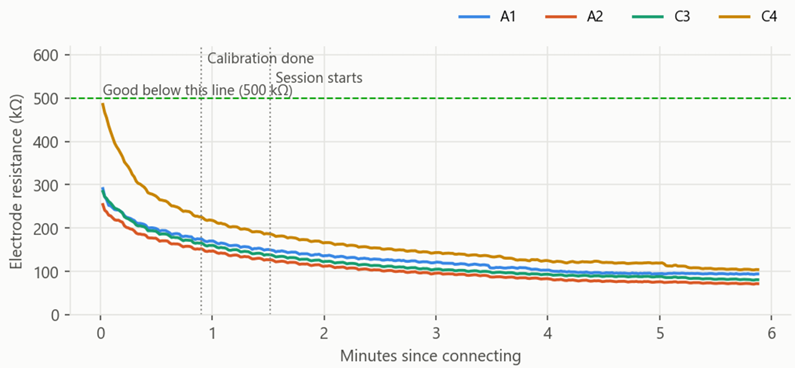
\includegraphics[width=0.8\linewidth]{electrode_impedance.png}
    \caption{Electrode resistance of the four channels after connecting the headset}
    \label{fig:impedance}
\end{figure}

All four electrodes start between 250 and 500 k$\Omega$ and settle to between 70 and 110
k$\Omega$ within about four minutes, which is well inside the usable range. C4 settles
highest and takes longest, which is consistent with it being the channel that gave the
noisiest motor imagery traces. The figure also shows why the session is not started
immediately: calibration is performed at around one minute and the session begins at about
one and a half minutes, by which time the contact has largely stabilised.

Two filters are applied to the continuous signal before the band powers are computed. Their
responses are shown in Figure~\ref{fig:filter}. A 0.5 Hz high-pass filter removes the slow
drift caused by sweat and small movements of the electrodes while leaving the delta band
intact, and a 50 Hz notch filter removes mains interference. Both filters process the
signal block by block while keeping their internal state, so that no discontinuity is
introduced at the block boundaries.

\begin{figure}[!htbp]
    \centering
    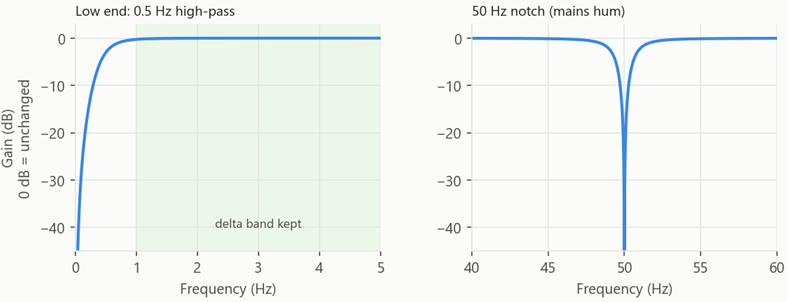
\includegraphics[width=0.8\linewidth]{filter_response.png}
    \caption{Frequency response of the 0.5 Hz high-pass and 50 Hz notch filters}
    \label{fig:filter}
\end{figure}

\FloatBarrier

\subsection{Usable Frequency Range}

Figure~\ref{fig:bandpower} shows how much of the original amplitude survives at each
frequency once the device filtering and the filters above are taken together.

\begin{figure}[!htbp]
    \centering
    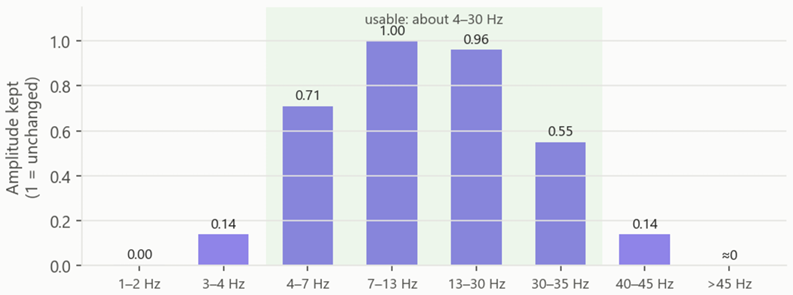
\includegraphics[width=0.8\linewidth]{normalized_band_power.png}
    \caption{Fraction of the original amplitude retained across frequency bands}
    \label{fig:bandpower}
\end{figure}

The 7--13 Hz and 13--30 Hz ranges pass almost unchanged, at 1.00 and 0.96, and the 4--7 Hz
range is retained at 0.71. Below 4 Hz the response falls away sharply, to 0.14 in the 3--4
Hz range and effectively to zero below 2 Hz, and above 35 Hz it falls away in the same way.
The practical consequence is that the delta band cannot be measured reliably with this
device and the gamma band is only partly available, so the effective measurement range for
cognitive scoring is about 4 to 30 Hz. The scores used in this work are therefore built
from theta, alpha and beta, which all lie inside that range.

\subsection{Stress and Fatigue Reference Levels}

Stress is estimated from the arousal ratio, which is the relative high-beta power in the
20--30 Hz range divided by the relative alpha power \cite{gelo2026manual}. When a person
becomes tense, beta
activity rises and alpha activity falls, so this ratio increases.
Figure~\ref{fig:arousal} shows how the ratio behaved over one session.

\begin{figure}[!htbp]
    \centering
    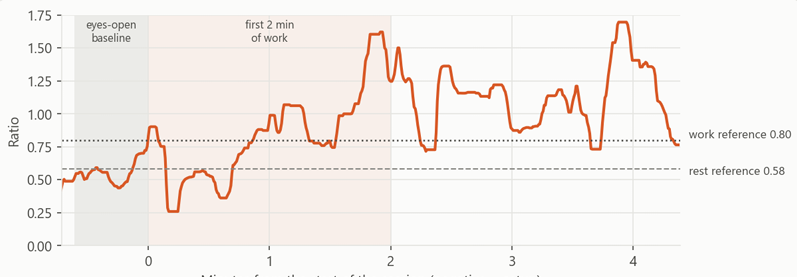
\includegraphics[width=0.8\linewidth]{arousal_ratio.png}
    \caption{Arousal ratio over a session, with the rest and work reference levels marked}
    \label{fig:arousal}
\end{figure}

During the eyes-open baseline the ratio stays near 0.5, and a rest reference of 0.58 is
established from this period. Once work begins the ratio rises and moves between about 0.75
and 1.70 for the rest of the session. A work reference of 0.80 is taken from the first two
minutes of work, which are deliberately excluded from the stress calculation so that the
settling-in period is not reported as stress. The score itself is obtained by comparing the
current ratio against this reference,

\begin{equation}
\mathrm{Score} = 50 + 50 \tanh \left( \log_2 \frac{\mathrm{ratio}}{\mathrm{reference}} \right)
\end{equation}

which maps the ratio onto a 0 to 100 scale, with 50 meaning the person is at their own
reference level. The displayed value is the median over the last 30 seconds, so that a
single noisy block does not move the score. Fatigue is computed in the same way from the
ratio of combined theta and alpha power to beta power.

\FloatBarrier

\subsection{Complete Session Output}

Figure~\ref{fig:gui_cognitive} shows the interface at the end of a monitoring session, with
all the outputs computed from the single four-channel recording.

\begin{figure}[!htbp]
    \centering
    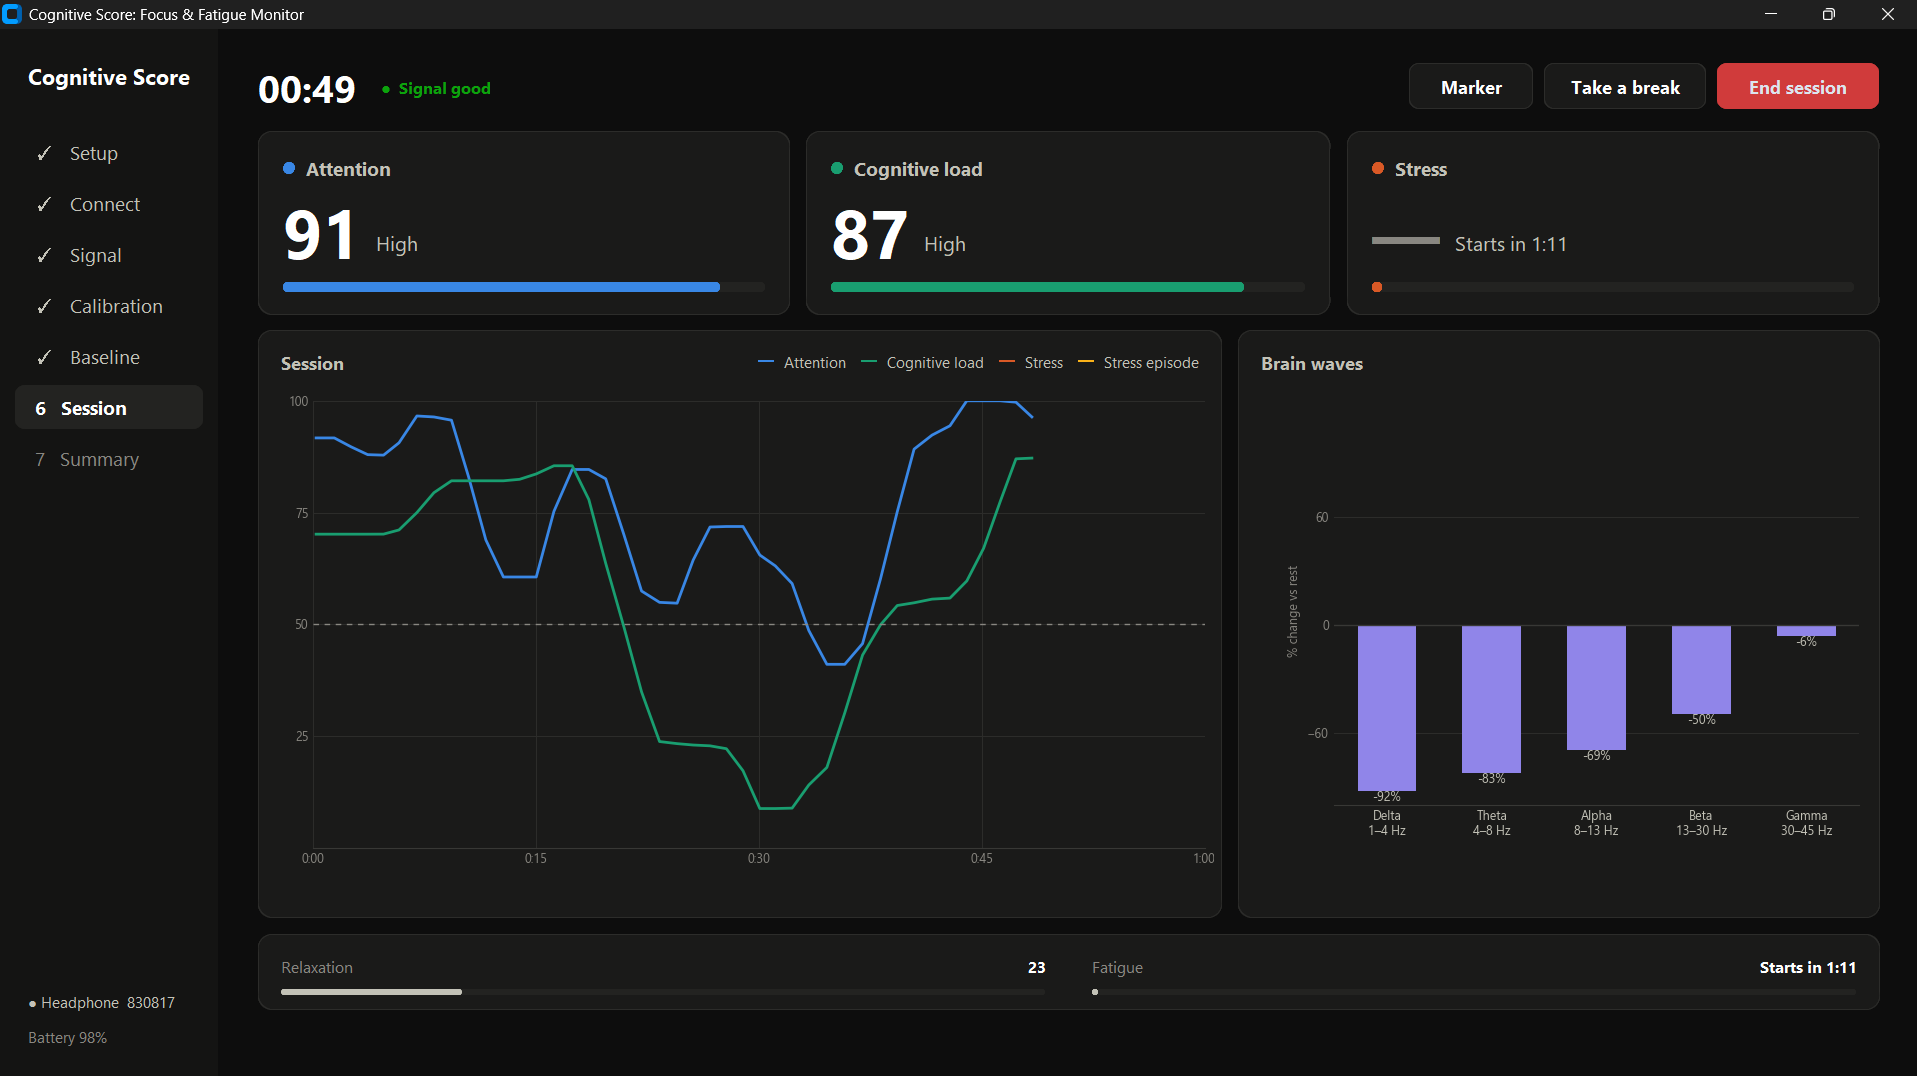
\includegraphics[width=\linewidth]{gui_cognitive_score.png}
    \caption{Cognitive score interface showing the session output}
    \label{fig:gui_cognitive}
\end{figure}

At the instant captured, attention is 91 and cognitive load is 87, both reported as high,
while relaxation is 23. Stress and fatigue are shown as not yet available, since both
require the opening period of the session to pass before a reference can be established.
The session plot in the middle shows how attention and cognitive load changed over the
minute of recording. The two do not move together throughout: around the half minute mark
cognitive load drops to near 10 while attention stays above 40, and both then climb back
together towards the end. This is useful because it shows the two measures are not simply
reporting the same quantity under different names.

The brain wave panel on the right shows the change in each band relative to the resting
baseline. Delta is down 92 per cent, theta down 83 per cent, alpha down 69 per cent, beta
down 50 per cent and gamma down 6 per cent. The pattern is consistent with an alert,
engaged state, since the slow bands associated with drowsiness are suppressed much more
than the faster bands associated with active thinking. The delta figure should not be read
too closely, as Figure~\ref{fig:bandpower} shows that very little of the delta band survives
the filtering on this device.

The sidebar also shows that the session follows a fixed sequence of setup, connection,
signal check, calibration, baseline and then the session itself, and the signal quality
indicator stayed green throughout, confirming that the contact held for the full recording.

\FloatBarrier

\section{Reason for the Observed Variations}

The differences seen between the two motor imagery classes come from the way the motor
cortex is organised. Imagining a movement of one hand changes the activity over the
opposite hemisphere, so the balance of power between C3 and C4 shifts depending on which
hand is imagined. This is what both the ERD traces in Figure~\ref{fig:erd_ours} and the
power ratios in Figures~\ref{fig:psd_left} and~\ref{fig:psd_right} show, and it is the only
property of the signal that separated the two classes reliably in this work.

The difference between the recorded data and the reference dataset has two main causes. The
headset used here has four dry electrodes while the reference system had thirty saline
electrodes, so both the signal quality and the amount of spatial information available are
lower. The baseline used for the ERD calculation is also taken from the moments just before
the marker, when the subject is already preparing for the task, so it does not represent a
true rest level and the computed percentages are shifted upward as a result.

The low classification accuracy follows from the same two causes, together with the decision
to train on one dataset and test on another. The subjects differ, the recording hardware
differs, the sampling rate differs and the number of channels differs, so features computed
on the training set do not fall in the same range as those computed on the test set. The
small amount of recorded data, 50 right-hand and 22 left-hand usable trials, also means the
two classes are unbalanced, which pushes a classifier towards the majority class and keeps
the accuracy near the chance level.

For the cognitive scoring, the variation between sessions is handled by referencing
everything to the person's own calibration. Because the scores are computed from relative
band powers and compared against a baseline recorded at the start of each session, a change
in overall signal level caused by electrode contact improving or worsening does not by
itself change the score.

The BCI Competition IV 2b data shows a different kind of variation, between people
rather than between devices. All nine subjects show the expected change in the C3/C4
balance, but its size differs a lot, from a ratio of 2.28 against 0.70 for B04 to 0.91
against 0.83 for B02. The overall level of the ratio also differs, so that for some
people both values sit above 1 and for others both sit below 1. This is most likely due
to the exact
position of the electrodes over each person's motor cortex, the shape of the head and how
strongly each person can imagine the movement, and it is the reason the decision threshold has to
be learned for each person or the data aligned first.

\section{Summary of Analysis}

The BCI Competition IV 2b dataset confirms that the analysis method and the classifiers
used in this project work. With the same ERD/ERS recipe as for the stroke patients, the
channel opposite to the imagined hand drops more in 16 of 18 cases, and subject B04 shows a
textbook pattern, with C4 falling to about $-50$ per cent for left-hand imagery and C3 to
about $-60$ per cent for right-hand imagery. The C3/C4 power ratio is higher for the left
hand than for the right hand in all nine subjects, and as a single number it identifies
the hand on unseen days with 73.5 per cent accuracy, better than chance for every subject
and 96.6 per cent for B04. The best SVM reached 80.2 per cent when trained on the same
person and 74.7 per cent on a new person, and the model choice mattered far less than
Euclidean alignment or the quality of the data.

The recorded GELO data shows the same kind of difference in the examples analysed, with
the C3 to C4 power ratio reaching 9.52 for a left-hand trial and 0.86 for a right-hand
trial on the same subject, and the direction of the difference between the two channels
reversing between the classes. Taken over all 72 recorded trials, however, the difference
is much weaker than in the 2b data.

The classifiers trained on the stroke data and tested on the recorded data do not convert
this difference into useful accuracy. All six
combinations of feature set and kernel gave between 50 and 54 per cent on a two-class
problem. Since the published benchmarks on the reference dataset reach only 55 to 72 per
cent using thirty channels and matched training and test conditions, the result is in line
with the difficulty of the problem, but it confirms that training on a public dataset and
testing on data from a different device is not a workable strategy. The same conclusion
holds for a model trained on the BCI Competition IV 2b data, which works well on new 2b
subjects but not on the recorded trials. The next step is to
record a larger and better balanced set of trials on the headset itself and to train and
test within that data, rather than across the two sources.

The cognitive assessment part of the system is working end to end. Electrode impedance
settles into the usable range within a few minutes, the filtering gives a reliable
measurement band of roughly 4 to 30 Hz, and attention, cognitive load, relaxation, stress
and fatigue are computed from the band powers and displayed live against the person's own
calibrated reference. The session output in Figure~\ref{fig:gui_cognitive} shows attention
and cognitive load varying independently over a recording, which indicates that the scores
are responding to the signal rather than tracking a single underlying quantity.

\section{Work carried out so far}

The work completed so far covers the following stages. A review of existing research was
carried out on EEG signal processing, motor imagery decoding, frequency band analysis and
machine learning methods for EEG, and the approach for the project was decided on the basis
of that review. The hardware was then set up using the GELO BCI headset, and a recording
procedure was established covering electrode impedance checking, alpha peak calibration,
baseline calibration and marker placement.

The ERD/ERS analysis reported in the reference dataset was reproduced to confirm that the
processing chain was correct, after which EEG data was recorded for left-hand and
right-hand motor imagery and the same analysis applied to it. The channels involved in left
and right motor imagery were identified, and the recorded data was compared against the
published results. The same analysis was then carried out on all nine subjects of the BCI
Competition IV 2b dataset, covering ERD/ERS, PSD, the C3/C4 power ratio and a set of SVM and
CSP classifiers tested on later sessions and on new people, and a 2b model was tested on
the recorded data. Several SVM models were then trained using different feature sets and
kernels, and the features that separate the two classes were identified. In parallel, the
cognitive scoring system was built and tested over complete sessions, covering calibration,
band power computation, score calculation and the display interface.